\graphicspath{{chapters/deep_learning/}}

\chapter{Deep CCA and Self-Supervised Learning: Non-Linear Functions}\label{ch:deep_learning}
\minitoc
% chktex-file 44
% chktex-file 3
\section*{Preface}

This chapter is based on work presented in \citet{chapman2023cca} and \citet{chapman2023efficient}.

\section{Introduction}

Deep CCA \citep{andrew2013deep} secured a runner-up position for the test-of-time award at ICML 2023 \citep{ICML2023TOT}.
However, its direct application has been limited in large datasets due to biased gradients in the stochastic minibatch setting.
There have since been proposals to scale-up Deep CCA in the stochastic case with adaptive whitening \citep{wang2015stochastic} and regularization \citep{chang2018scalable}, but these techniques are highly sensitive to hyperparameter tuning.

Self-Supervised Learning (SSL) methods have reached the state-of-the-art in tasks such as image classification \citep{balestriero2023cookbook}, learning representations without labels that can be used to classify images using a linear probe in the zero-shot setting.
A family of SSL methods that are closely aligned with Canonical Correlation Analysis (CCA) has garnered particular interest.
This family notably includes Barlow Twins \citep{zbontar2021barlow}, VICReg \citep{bardes2021vicreg}, and W-MSE \citep{ermolov2021whitening} and they aim to transform a pair of data views into similar representations, similar to the objective of CCA. Similarly, some generative approaches to SSL\citep{sansone2022gedi} bear a striking resemblance to Probabilistic CCA\citep{bach2005probabilistic}.
These connections have started to be explored in \citet{balestriero2022contrastive}.

In this chapter, we propose a novel formulation of Deep CCA that is unbiased in the stochastic setting and scales to large datasets.
We also propose a novel SSL method, SSL-EY, that is competitive with existing methods on CIFAR-10 and CIFAR-100.
We highlight the connections between our work and existing SSL methods, and show that our method is more robust to hyperparameter tuning.

\section{Background: Deep Representation Learning}

\subsection{Deep Learning}

Deep learning is a subfield of machine learning that uses functions parameterised by neural networks.
Deep learning has been applied to a wide range of domains, including computer vision, speech recognition, natural language processing, and bioinformatics, where they have produced state-of-the-art results on many tasks.
Neural networks are usually composed of many linear layers followed by nonlinear activation functions such as the rectified linear unit (ReLU).
The ReLU activation function is defined as $\ReLU(x) = \max(0, x)$.
The ReLU activation function is piecewise linear, and so the composition of ReLU activations with linear functions is a piecewise linear function.
It has been shown that neural networks with ReLU activations can approximate any continuous function on a compact set to arbitrary accuracy \citep{perekrestenko2018universal}, and so are universal function approximators.
This flexibility, combined with increasingly large datasets, allows neural networks to learn complex functions from data.
Owing to the size of the models and datasets, neural networks are usually trained using the backpropagation algorithm and stochastic gradient descent (SGD) \citep{amari1993backpropagation}.

\subsection{DCCA and Deep Multiview CCA}

Thus far, our focus in this thesis has been on linear CCA. However, in dealing with high-dimensional and complex data structures commonly found in modern applications, nonlinear extensions of CCA become essential.
The objective of DCCA and DMCCA is to learn nonlinear representations of data that are linearly correlated across different views. Recall the definition of $\MCCA_K$ in Equation \eqref{eq:MCCA}. We define the goal of DCCA and DMCCA using this notation:

\begin{align}
\label{eq:DMCCA-def}
\norm{\MCCA_K\left(Z^{(1)}, \ldots, Z^{(I)}\right)}_2
\end{align}

which is the norm of the vector of the top $K$ canonical correlations between the representations $Z^{(i)}$ of the different views.

The key difference between MCCA and its deep learning counterparts, DCCA and DMCCA, lies in the nature of the input data. In MCCA, we work with fixed, pre-defined feature representations $X^{(i)}$ for each view and aim to find linear transformations that maximize the correlation between these fixed representations. In contrast, DCCA and DMCCA learn new, nonlinear representations $Z^{(i)} = f^{(i)}(X^{(i)}; \theta^{(i)})$ using neural networks $f^{(i)}$ parameterized by $\theta^{(i)}$ for each view $i \in [I]$. The objective is to learn representations that have high MCCA, i.e., representations that are maximally correlated across views in a linear sense.

The power of DCCA and DMCCA lies in their ability to learn flexible, nonlinear transformations of the input data that are tailored to the task of maximizing cross-view correlation. By learning these representations end-to-end, DCCA and DMCCA can potentially capture more complex and subtle relationships between views that may be difficult or impossible to capture with fixed, linear transformations.

\begin{figure}
\centering
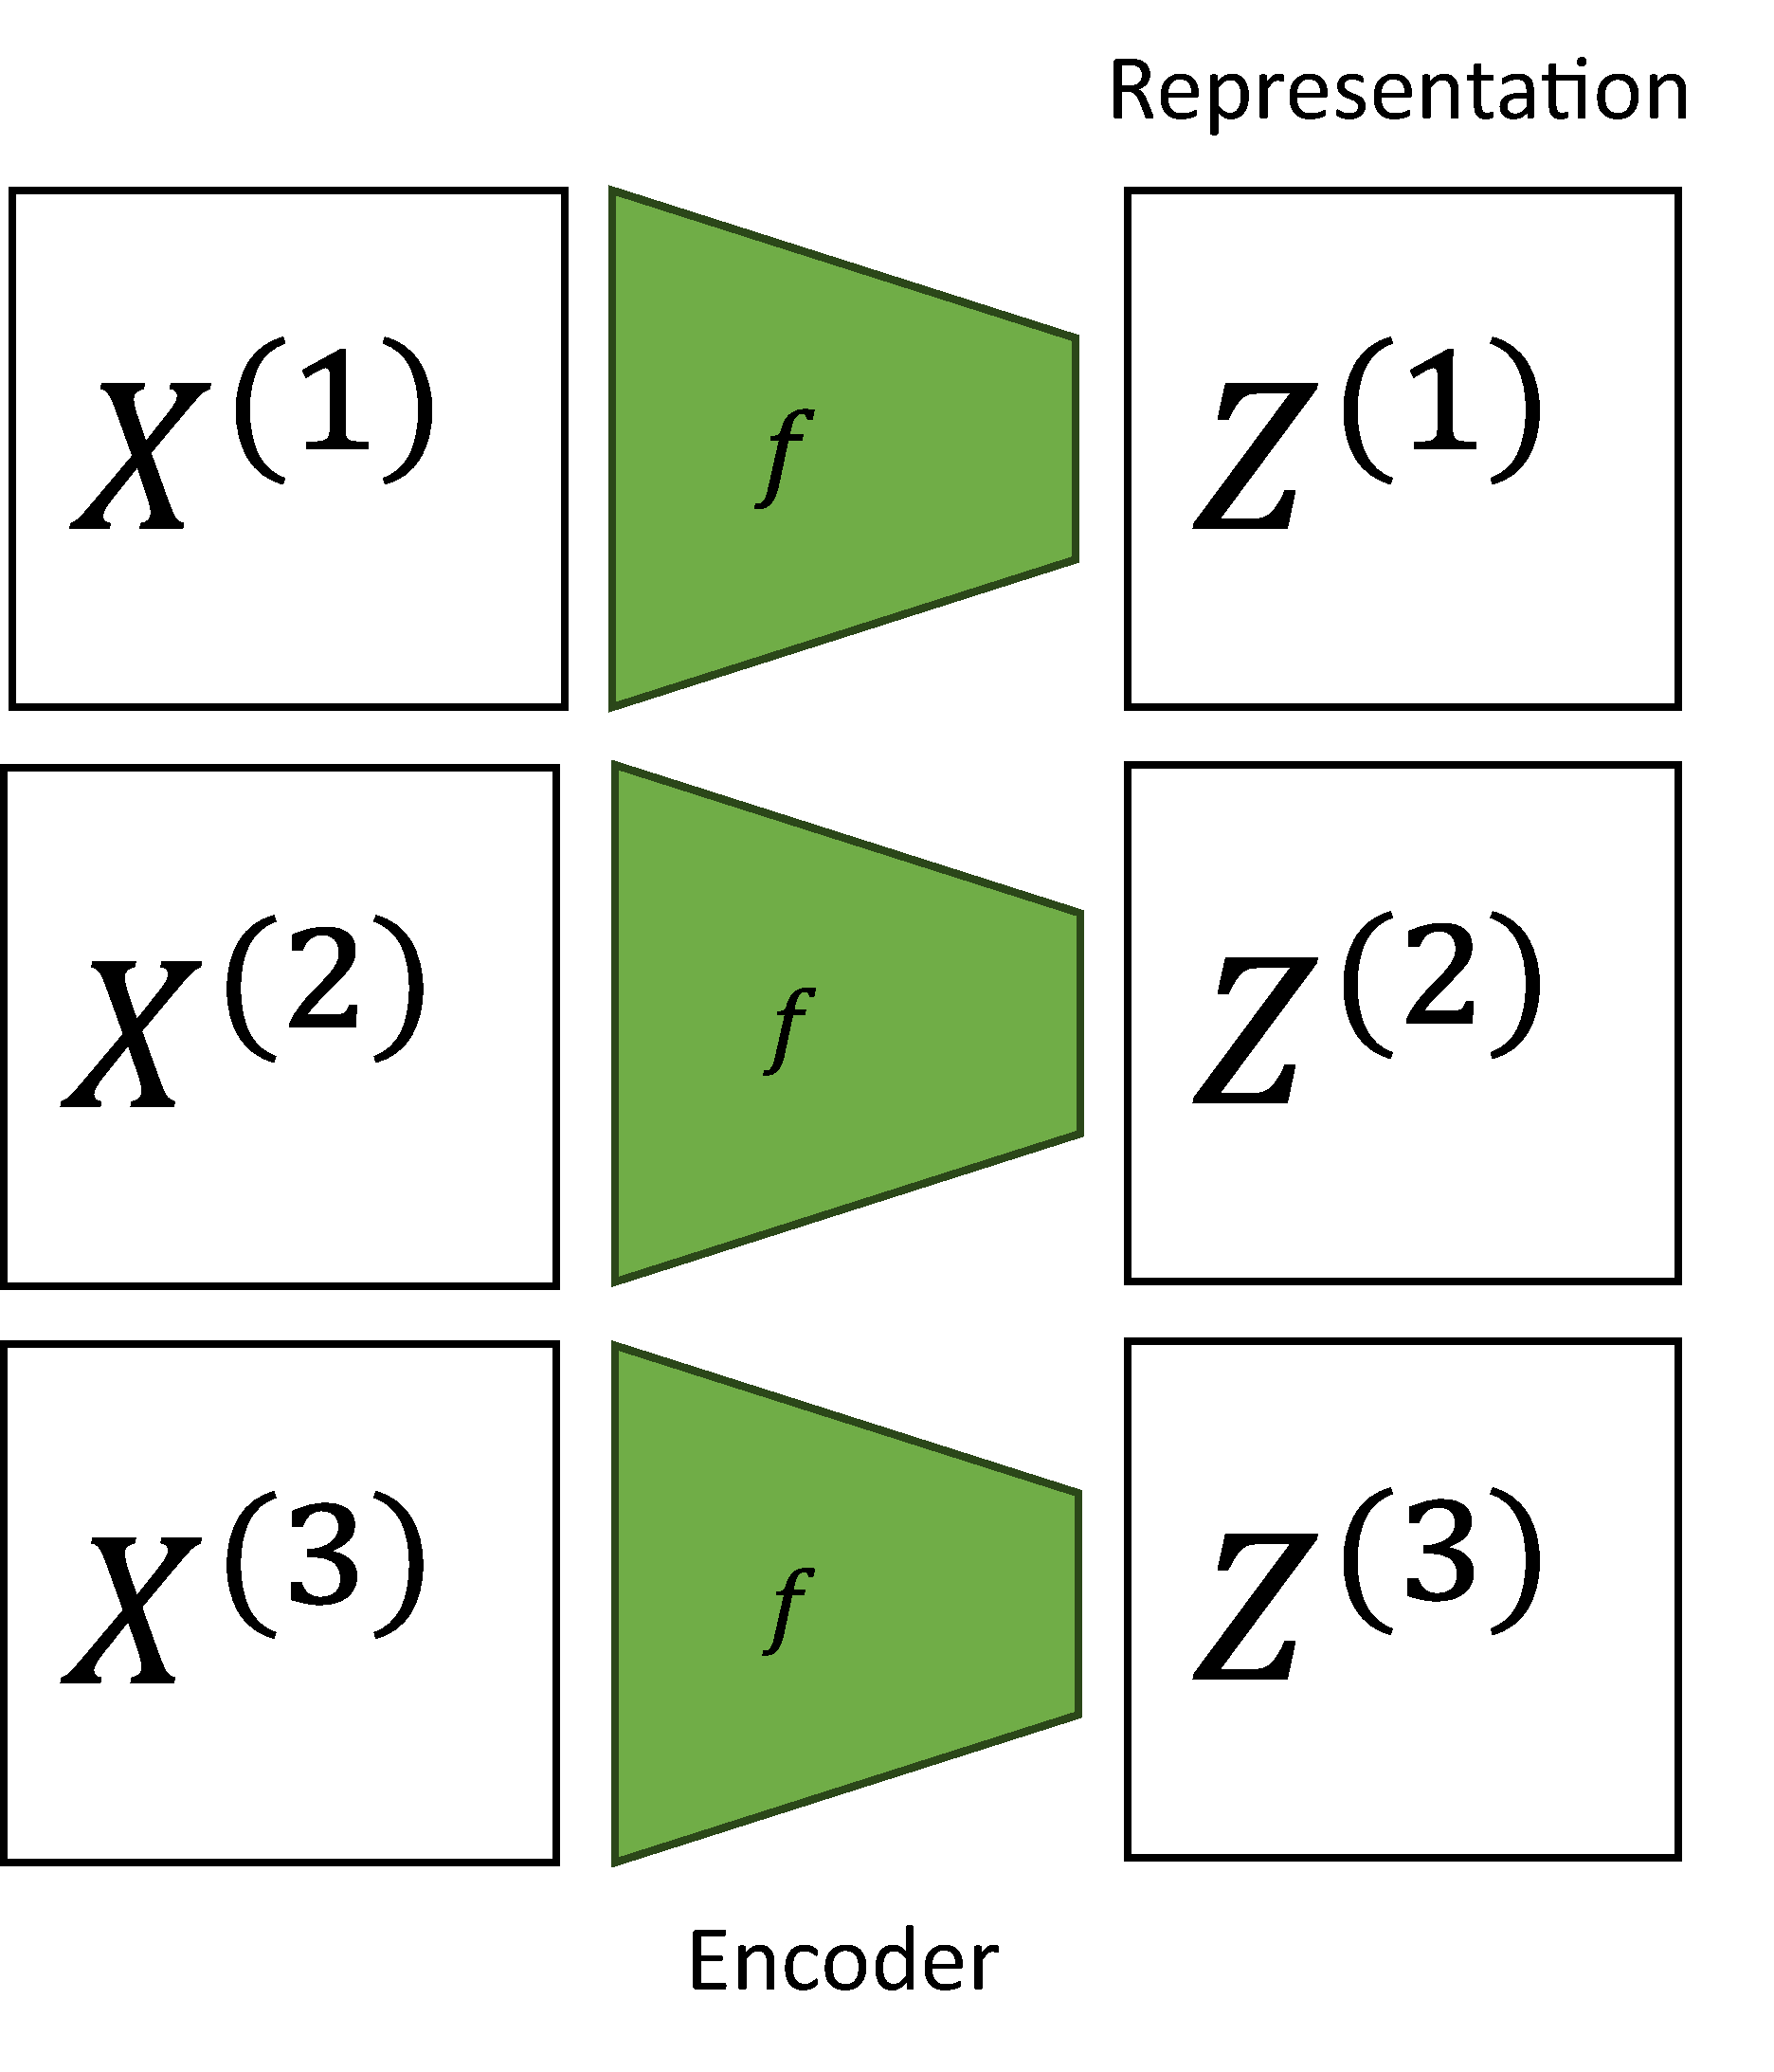
\includegraphics[width=0.5\textwidth]{figures/dcca_schematic}
\caption{Schematic of the DCCA approach highlighting the nonlinear transformation of data into correlated views.}
\label{fig:dcca_schematic}
\end{figure}

Figure \ref{fig:dcca_schematic} illustrates the conceptual framework of DCCA, where data from different views are transformed through neural networks to achieve correlated representations.

The full-batch approach of DCCA, formulated by \citet{andrew2013deep}, seeks to maximize the correlation between these different views.
The objective, operationalized as a loss function, is defined by the trace of matrix $T$:
\begin{align}\label{eq:T_definition}
T &= \left(\text{cov}(Z^{(1)})\right)^{-\frac{1}{2}} Z^{(1)\top} Z^{(2)} \left(\text{cov}(Z^{(2)})\right)^{-\frac{1}{2}} \\
\LRayleigh &= -\Tr(T)
\end{align}

This approach, while theoretically sound, faces scalability issues with large datasets.
DCCA-STOL, proposed by \citet{wang2015unsupervised}, adapts this objective to large mini-batches but suffers from biased gradients due to the matrix inversions in Equation \eqref{eq:T_definition}.
This necessitates batch sizes larger than the representation size, limiting its practical application.

Extensions such as DMCCA \citep{somandepalli2019multimodal} and DGCCA \citep{benton2017deep} are multiview extensions of DCCA that work by directly differentiating the sum of the top $K$ generalized eigenvalues of the mini-batch covariance matrices. Specifically, their loss function is given by:
\begin{align}
    T &= \left(\hat{V}(\theta)^{-\frac{1}{2}} \hat{C}(\theta)\hat{V}(\theta)^{-\frac{1}{2}}\right)\\
    \LMCCA &= -\Tr(T)
\end{align}
    where $\hat{C}(\theta)$ and $\hat{V}(\theta)$ are the mini-batch estimates of the between-view and within-view covariance matrices, respectively, as defined in Equation \eqref{eq:def-C-V-matrices}.

However, these methods suffer from the same fundamental issue as DCCA-STOL, namely the biased gradients resulting from the eigendecomposition of small mini-batch covariance matrices. As a result, DMCCA and DGCCA do not effectively mitigate the scalability issues of DCCA and still require large batch sizes to work well in practice.

Adaptive whitening methods \citep{wang2015stochastic, chang2018scalable} offer another solution by reducing the bias in the DCCA objective.
However, as noted in DCCA-NOI \citep{wang2015unsupervised}, these methods introduce a time constant that complicates analysis and requires extensive tuning:
\begin{align}
\LNOI &= |{\tilde{\Sigma}_{11}}^{-\frac{1}{2}} Z\sps{1}-{\tilde{\Sigma}_{22}}^{-\frac{1}{2}} Z\sps{2}|^2_F
\end{align}
where $\tilde{\Sigma}_{11}$ and $\tilde{\Sigma}_{22}$ are estimates of the covariance matrices of $Z\sps{1}$ and $Z\sps{2}$, respectively.

These limitations highlight the need for more scalable and efficient nonlinear CCA methods that can handle large datasets without compromising on representation quality or requiring extensive hyperparameter tuning.

\subsection{Self-Supervised Learning and Joint Embedding}

Self-Supervised Learning (SSL) has emerged as a crucial approach in deep learning, especially for tasks with limited labeled data. A fundamental strategy in SSL, particularly in non-contrastive SSL, involves creating joint embeddings of augmented images. This process entails generating two distinct views of the same image, denoted as \( X_1 \) and \( X_2 \), using various augmentation techniques. The primary aim is to align their representations, \( Z^{(1)} \) and \( Z^{(2)} \), in a shared embedding space. This alignment leverages the inherent patterns within the data to develop feature representations absent explicit labels. A significant challenge in this methodology is averting the collapse of representations, where models produce constant features irrespective of input variability.

\begin{figure}[ht]
    \centering
    \tikz{ % nodes
        \node[latent, align=center, minimum size=2cm] (x) {Original Image\\x};
        \node[obs, below left=of x, minimum size=2cm, align=center] (x1) {Augmented Image \\$x^{(1')}$};
        \node[obs, below right=of x, minimum size=2cm, align=center] (x2) {Augmented Image \\$x^{(2')}$};
        % edges
        \edge{x} {x1}
        \edge{x} {x2}}
    \caption[Joint Embedding Data Generation Process]{\textit{\textbf{Joint Embedding Data Generation Process:}} The original image \(x\) is augmented to produce two views \(x^{(1')}\) and \(x^{(2')}\).}
    \label{fig:joint-embedding}
\end{figure}

In SSL, augmented data generation serves to create multiple perspectives of the same underlying content, such as cropping or rotating an image. The objective is to learn representations that are invariant to these augmentations, thereby capturing the fundamental structure of the data. Canonical Correlation Analysis (CCA) emerges as a fitting tool for this task, especially given that augmentations represent redundant rather than complementary information, offering different perspectives of the same underlying data.

\subsubsection{Encoder-Projector Model in SSL}
SSL methods like Barlow Twins and VICReg employ an encoder-projector model, as shown in Figure~\ref{fig:sslschematic}. In this model, input data is transformed by an encoder \( g \) into representations, which are further processed by a projector \( h \) into higher-dimensional embeddings. These embeddings are integral to training, with the representations being critical for downstream tasks. The encoder is typically a neural network suited to the domain, while the projector is often a simpler multi-layer perceptron.

\begin{figure}[ht]
    \centering
    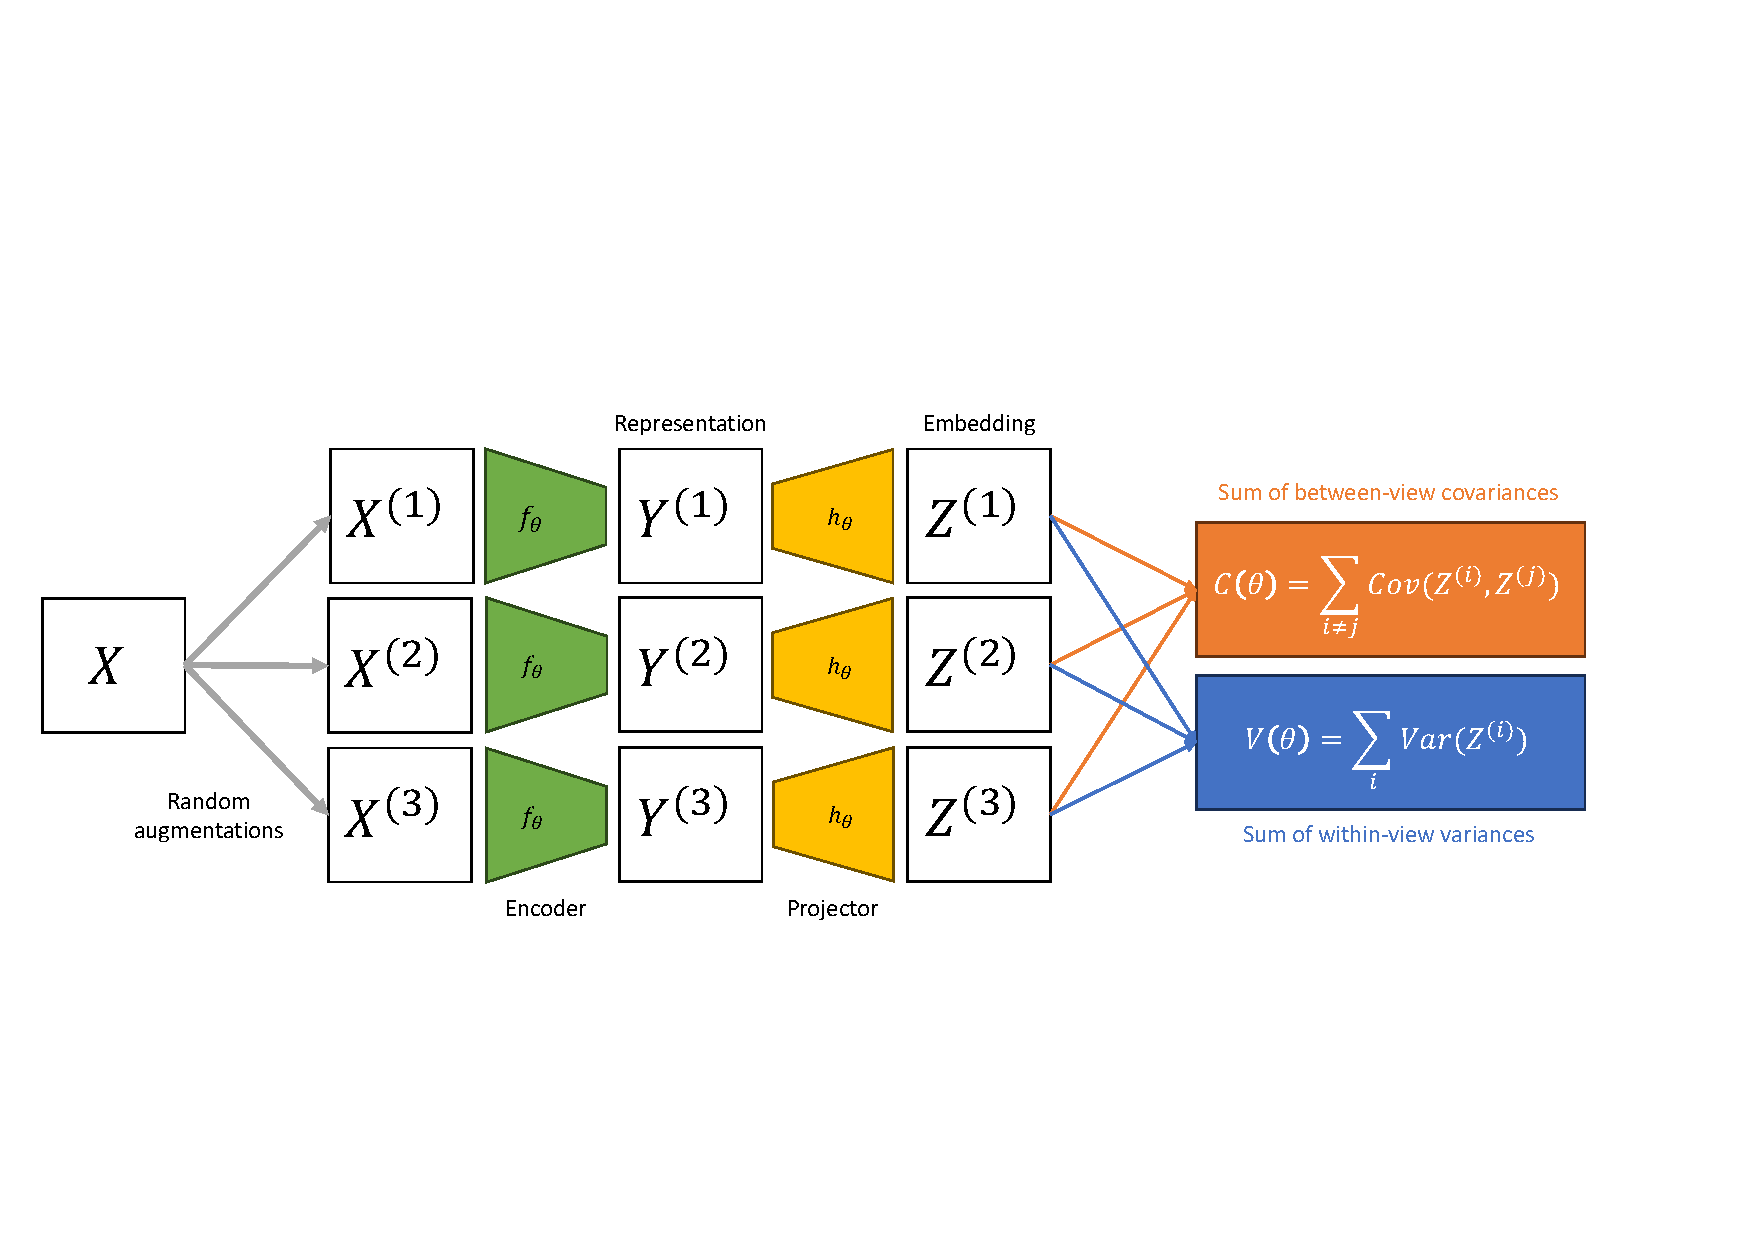
\includegraphics[width=0.99\textwidth]{figures/ssl_schematic}
    \caption{Schematic of the encoder-projector setup in SSL.}
    \label{fig:sslschematic}
\end{figure}

The essence of joint embedding in SSL is that similar inputs, \( X \) and its augmented version \( X' \), should yield similar embeddings, \( Z \) and \( Z' \).
The encoder and projector are optimized to minimize the distance between \( Z \) and \( Z' \), reflecting the similarity of the inputs.

\subsubsection{CCA-based SSL Methods: Barlow Twins and VICReg}
Barlow Twins and VICReg are two pivotal methods in SSL that build upon canonical correlation principles to generate robust representations from augmented views.
Both methods aim to align representations of two augmented views while ensuring distinct yet correlated representations.

\textbf{Barlow Twins} employs a redundancy reduction objective to ensure similarity between representations of the same augmented views and to decorrelate representations within each view.
Its loss function is expressed as:
\begin{align}
    \LBT = \overbrace{\gamma \mathbb{E} \norm{Z^{(1)} - Z^{(2)}}^2}^{\text{Invariance}} + \overbrace{\beta \sum_{\substack{k,l=1 \\ k \neq l}}^K \Cov(\hat{Z}^{(i)}_k, \hat{Z}^{(i)}_l)^2}^{\text{Redundancy Reduction}},
\end{align}
where \( \hat{Z}^{(i)} \) denotes the batch-normalized versions of the representations, with \( \gamma \) and \( \beta \) as hyperparameters controlling the similarity and decorrelation terms, respectively.

\textbf{VICReg}, in contrast, introduces a variance term and omits batch normalization, focusing on variance-invariance-covariance regularization.
The VICReg loss is defined as:
\begin{align}
    \LVR = \overbrace{\gamma \mathbb{E} \norm{Z^{(1)} - Z^{(2)}}^2}^{\text{Invariance}} + \left[\overbrace{\sum_{i \in \{1,2\}} \alpha \sum_{k=1}^K \left(1 - \sqrt{\Var(Z^{(i)}_k)}\right)_+}^{\text{Variance}} + \overbrace{\beta \sum_{\substack{k,l=1 \\ k \neq l}}^K \Cov(Z^{(i)}_k, Z^{(i)}_l)^2 }^{\text{Covariance}}\right],
\end{align}
with \( \alpha \), \( \beta \), and \( \gamma \) as tuning parameters balancing the influence of variance, invariance, and covariance regularization.

These approaches, grounded in canonical correlation principles, offer foundational baselines for our experiments in SSL.


\section{Methods: Novel Objectives and Algorithms}

Recall the definition of our family of objectives from definition \ref{def:EY-objectives}.
We will now consider non-linear transformations of the data $Z\sps{i} = f\sps{i}( X\sps{i}; \theta\sps{i})$, and show that our objectives are well-suited to this setting.

\subsection{Applications to (multi-view) Deep CCA}

We first show that our objective recovers Deep Multi-view CCA at any local optimum, assuming a final linear layer in each neural network.

\begin{restatable}{lemma}{recoverDeepCCA}[Objective recovers Deep Multi-view CCA]\label{lem:recover-DeepCCA}
Assume that there is a final linear layer in each neural network $f\sps{i}$.
Then at any local optimum, $\hat{\theta}$, of the population problem, we have
\begin{align*}
\LEY(\hat{\theta}) = - \norm{\MCCA_K(\hat{Z})}_2^2
\end{align*}
where $\hat{Z} = f_{\hat{\theta}}(X)$.
Therefore, $\hat{\theta}$ is also a local optimum of objectives from \citet{andrew2013deep, somandepalli2019multimodal} as defined in \cref{eq:DMCCA-def}.
\end{restatable}

\begin{proof}[Proof sketch: see \cref{supp:EY-recover-Deep-CCA} for full details.]
Consider treating the penultimate-layer representations as fixed, and optimising over the weights in the final layer.
This is precisely equivalent to optimising the Eckhart-Young loss for linear CCA where the input variables are the penultimate-layer representations.
So by \cref{prop:no-spurious}, a local optimum is also a global optimum, and by \cref{prop:EY-charac} the optimal value is the negative sum of squared generalised eigenvalues.
\end{proof}

This result shows that our objective, which we call \textbf{DCCA-EY}, is a valid generalization of Deep CCA and can be used to learn correlated non-linear representations.

\subsection{Application to Self-Supervised Learning (SSL)}

We can directly apply Algorithm~\ref{alg:general} to the SSL setting by treating the two augmented views as different data views. We will refer to this method as \textbf{SSL-EY}.

If we wish to have the same neural network transforming each view, we can simply tie the weights $\theta\sps{1} = \theta\sps{2}$. When the paired data are generated from applying independent, identically distributed (i.i.d.) augmentations to the same original input, it is intuitive that tying the weights is a sensible procedure and may act as a regularizer\footnote{Given the distributions of both views are identical, there is no reason we would expect assymetric functions to be optimal out of sample}.

Moreover, our loss function bears some resemblance to those of Barlow Twins and VICReg. Recall that our objective is:

\begin{align*}
\LEY(\theta) = - 2 \tr C(\theta) + \norm{V_\alpha(\theta)}_F^2
\end{align*}

where $C(\theta)$ is the cross-covariance matrix between the representations of the two views, and $V_\alpha(\theta)$ is a matrix involving the individual covariance matrices of each view.

This objective has two terms: the first term, $- 2 \tr C(\theta)$, encourages the representations to be correlated across views, similar to the invariance term in Barlow Twins and VICReg. The second term, $\norm{V_\alpha(\theta)}_F^2$, involves the individual covariance matrices, which is analogous to the variance and covariance terms in VICReg. The main difference is that our method is based on canonical correlation principles, which may offer additional benefits in terms of representation quality and interpretability.

In the next section, we will present experiments demonstrating the effectiveness of our method in both the Deep CCA and SSL settings.

subsection{PyTorch Implementation}

We provide PyTorch implementations of DCCA-EY and SSL-EY in Listings \ref{lst:pytorch-dcca} and \ref{lst:pytorch-ssl}, respectively.

The DCCA-EY implementation defines a class that takes a list of encoders as input and computes the loss function as described in Section 3.2. The forward method computes the representations of the input data using the encoders, while the loss method computes the loss function based on the representations. This implementation can be used to train DCCA-EY models on multi-view data.

The SSL-EY implementation defines a class that takes a single encoder as input, which is used to transform both augmented views of the data. The forward method computes the representations of the input data using the shared encoder, while the loss method computes the loss function based on the representations and the ridge penalty hyperparameters. This implementation can be used to train SSL-EY models on augmented data.

In the next section, we will present experiments demonstrating the effectiveness of our DCCA-EY and SSL-EY methods in their respective settings.

\begin{listing}[ht]
    \begin{minted}{python}
    import torch
    import torch.nn as nn
    
    class DCCA_EY(nn.Module):
    def init(self, encoders):
    super(DCCA_EY, self).init()
    self.encoders = nn.ModuleList(encoders)
    def forward(self, Xs):
    Zs = [encoder(X) for encoder, X in zip(self.encoders, Xs)]
    return Zs

    def loss(self, Zs):
    # Compute total between-view covariance matrix
    C = torch.zeros(Zs[0].shape[1], Zs[0].shape[1])
    for i in range(len(Zs)):
        for j in range(i + 1, len(Zs)):
            C += torch.matmul(Zs[i].T, Zs[j]) / Zs[i].shape[0]
    
    # Compute total within-view variance matrix
    V = torch.zeros(Zs[0].shape[1], Zs[0].shape[1])
    for i in range(len(Zs)):
        V += torch.matmul(Zs[i].T, Zs[i]) / Zs[i].shape[0]
    
    # Compute loss
    loss = -2 * torch.trace(C) + torch.norm(V, p='fro') ** 2
    
    return loss
    \end{minted}
    \caption{PyTorch implementation of DCCA-EY.}    
    \label{lst:pytorch-dcca}
\end{listing}

We provide a PyTorch implementation of DCCA-EY in Listing \ref{lst:pytorch-dcca}. This implementation defines a DCCA-EY class that takes a list of encoders as input and computes the loss function as described in Section 3.2. The forward method computes the representations of the input data using the encoders, while the loss method computes the loss function based on the representations. This implementation can be used to train DCCA-EY models on multi-view data.

\begin{listing}[ht]
    \begin{minted}{python}
    import torch
    import torch.nn as nn
class SSL_EY(nn.Module):
def init(self, encoder):
super(SSL_EY, self).init()
self.encoder = encoder
def forward(self, Xs):
    Zs = [self.encoder(X) for X in Xs]
    return Zs

def loss(self, Zs, alphas=[0, 0]):
    # Compute cross-covariance matrix
    C = torch.matmul(Zs[0].T, Zs[1]) / Zs[0].shape[0]
    
    # Compute individual covariance matrices
    V1 = torch.matmul(Zs[0].T, Zs[0]) / Zs[0].shape[0]
    V2 = torch.matmul(Zs[1].T, Zs[1]) / Zs[1].shape[0]
    
    # Compute loss
    V_alpha = alphas[0] * torch.eye(V1.shape[0]) + (1 - alphas[0]) * V1 + \
              alphas[1] * torch.eye(V2.shape[0]) + (1 - alphas[1]) * V2
    loss = -2 * torch.trace(C) + torch.norm(V_alpha, p='fro') ** 2
    
    return loss
    \end{minted}
    \caption{PyTorch implementation of SSL-EY.}
    \label{lst:pytorch-ssl}
\end{listing}



\section{Experiments and Results}

\subsection{Deep CCA}\label{sec:experiments-DCCA}
In this experiment, we aim to establish the superiority of our DCCA-EY method over existing Deep Canonical Correlation Analysis (DCCA) approaches.
We specifically focus on showcasing how DCCA-EY outperforms these methods in terms of correlation capture, convergence speed, and ease of hyperparameter tuning.
The experimental setup is aligned with that of \citet{wang2015stochastic}, providing a direct comparison under identical conditions.

As per \citet{wang2015stochastic}, our architecture comprises multilayer perceptrons with two hidden layers of size 800 and an output layer of 50 with ReLU activations.
We train these networks for 20 epochs.
However, our primary goal is to learn $K=50$ dimensional representations over a range of mini-batch sizes (from 20 to 100) across 50 epochs, demonstrating the robustness and scalability of DCCA-EY even in varying batch conditions.

In this chapter, we employ the Total Correlation Captured (TCC) metric for evaluation.
While similar to the PCC metric described in the previous chapter, TCC does not rely on a ground truth for its computation.
Instead, it is defined as \( \text{TCC} = \sum_{k=1}^K \rho_k \), where $\rho_k$ are the empirical correlations between the neural network-based representations $Z^{(i)} = f^{(i)}(X^{(i)})$ on a validation set, rather than on the training set as was the case with PCC. This distinction is crucial as TCC evaluates the model's performance in capturing correlations in an unseen dataset, offering a more robust measure of its generalization capability.
\subsubsection{Data}
The Split MNIST dataset is a modified version of the original MNIST dataset, where each 28x28 pixel grayscale image of handwritten digits (0-9) is divided into left and right halves, creating two distinct views.
This split challenges models to learn from partial information, as each view contains only half of the digit, either the left or the right side.
The dataset comprises 50,000 training and 10,000 test images.
The X-Ray Microbeam Speech Production Database (XRMB) is a multi-view dataset used for studying articulatory speech data.
It comprises around 40,000 spoken utterances from 47 American English speakers.
The dataset provides two views: acoustic features and articulatory measurements.
The acoustic features consist of 273-dimensional vectors representing spectral characteristics, while the articulatory measurements include 112-dimensional vectors capturing the position and movement of speech articulators (like the tongue and lips).
The XRMB dataset is notable for its complexity and high dimensionality, making it a challenging testbed for multiview learning algorithms.

\subsubsection{Parameters} For each method, we searched over a hyperparameter grid using \citet{wandb}.

\begin{table}[h!]
    \centering
    \begin{tabular}{|l|l|}
        \hline Parameter           & Values           \\
        \hline minibatch size      & 100, 50, 20      \\
        \hline lr                  & 1e-3, 1e-4, 1e-5 \\
        \hline $\rho$\footnotemark & 0.6, 0.8, 0.9    \\
        \hline epochs              & 50               \\
        \hline
    \end{tabular}
    \footnotetext{$\rho$ is only used for DCCA-NOI}\label{tab:hyperparams}
\end{table}

\subsubsection{Observations on SplitMNIST}
For the SplitMNIST dataset, Figure~\ref{fig:corr_mnist} shows the comparison of methods across different batch sizes.
We observe that DCCA-STOL captures significantly less correlation than the other methods and breaks down when the mini-batch size is smaller than the dimension $K=50$.
Figure~\ref{fig:lr_mnist} illustrates the learning progress over 50 epochs, where DCCA-NOI, despite performing similarly to DCCA-EY, requires more careful hyperparameter tuning and demonstrates a slower convergence speed.

\subsubsection{Observations on XRMB}
On the XRMB dataset, as seen in Figure~\ref{fig:corr_xrmb}, similar trends are evident.
DCCA-STOL struggles with smaller mini-batch sizes, while DCCA-NOI, though comparable to DCCA-EY in performance, lags in convergence speed, as shown in Figure~\ref{fig:lr_xrmb}.

\begin{figure}
    \centering
    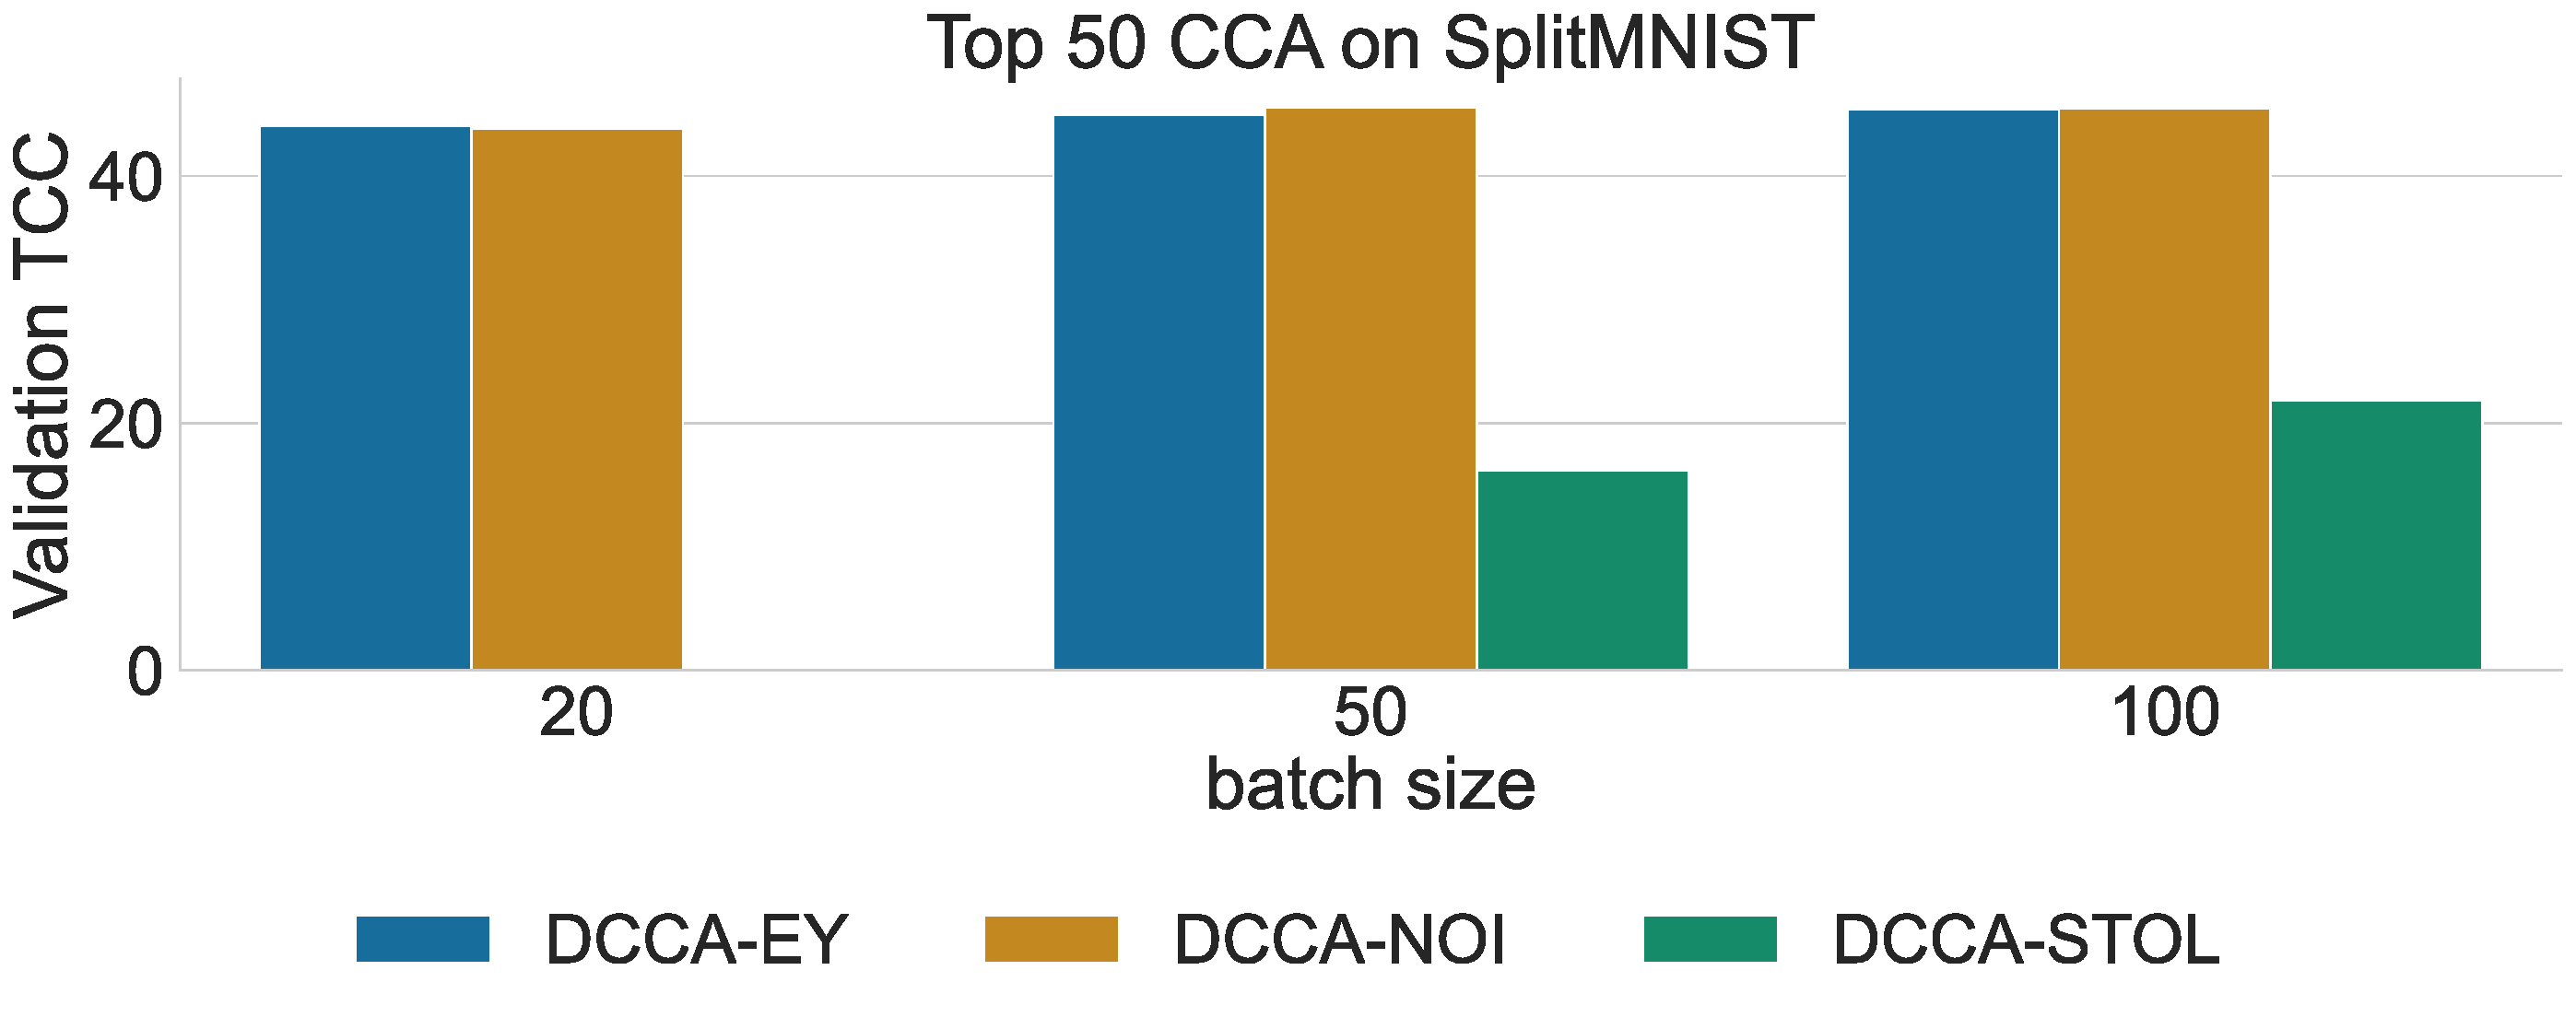
\includegraphics[width=0.8\textwidth]{figures/DCCA/SplitMNIST_models_different_batch_sizes}
    \caption{Deep CCA on SplitMNIST: Comparison of methods across varying batch sizes.}
    \label{fig:corr_mnist}
\end{figure}

\begin{figure}
    \centering
    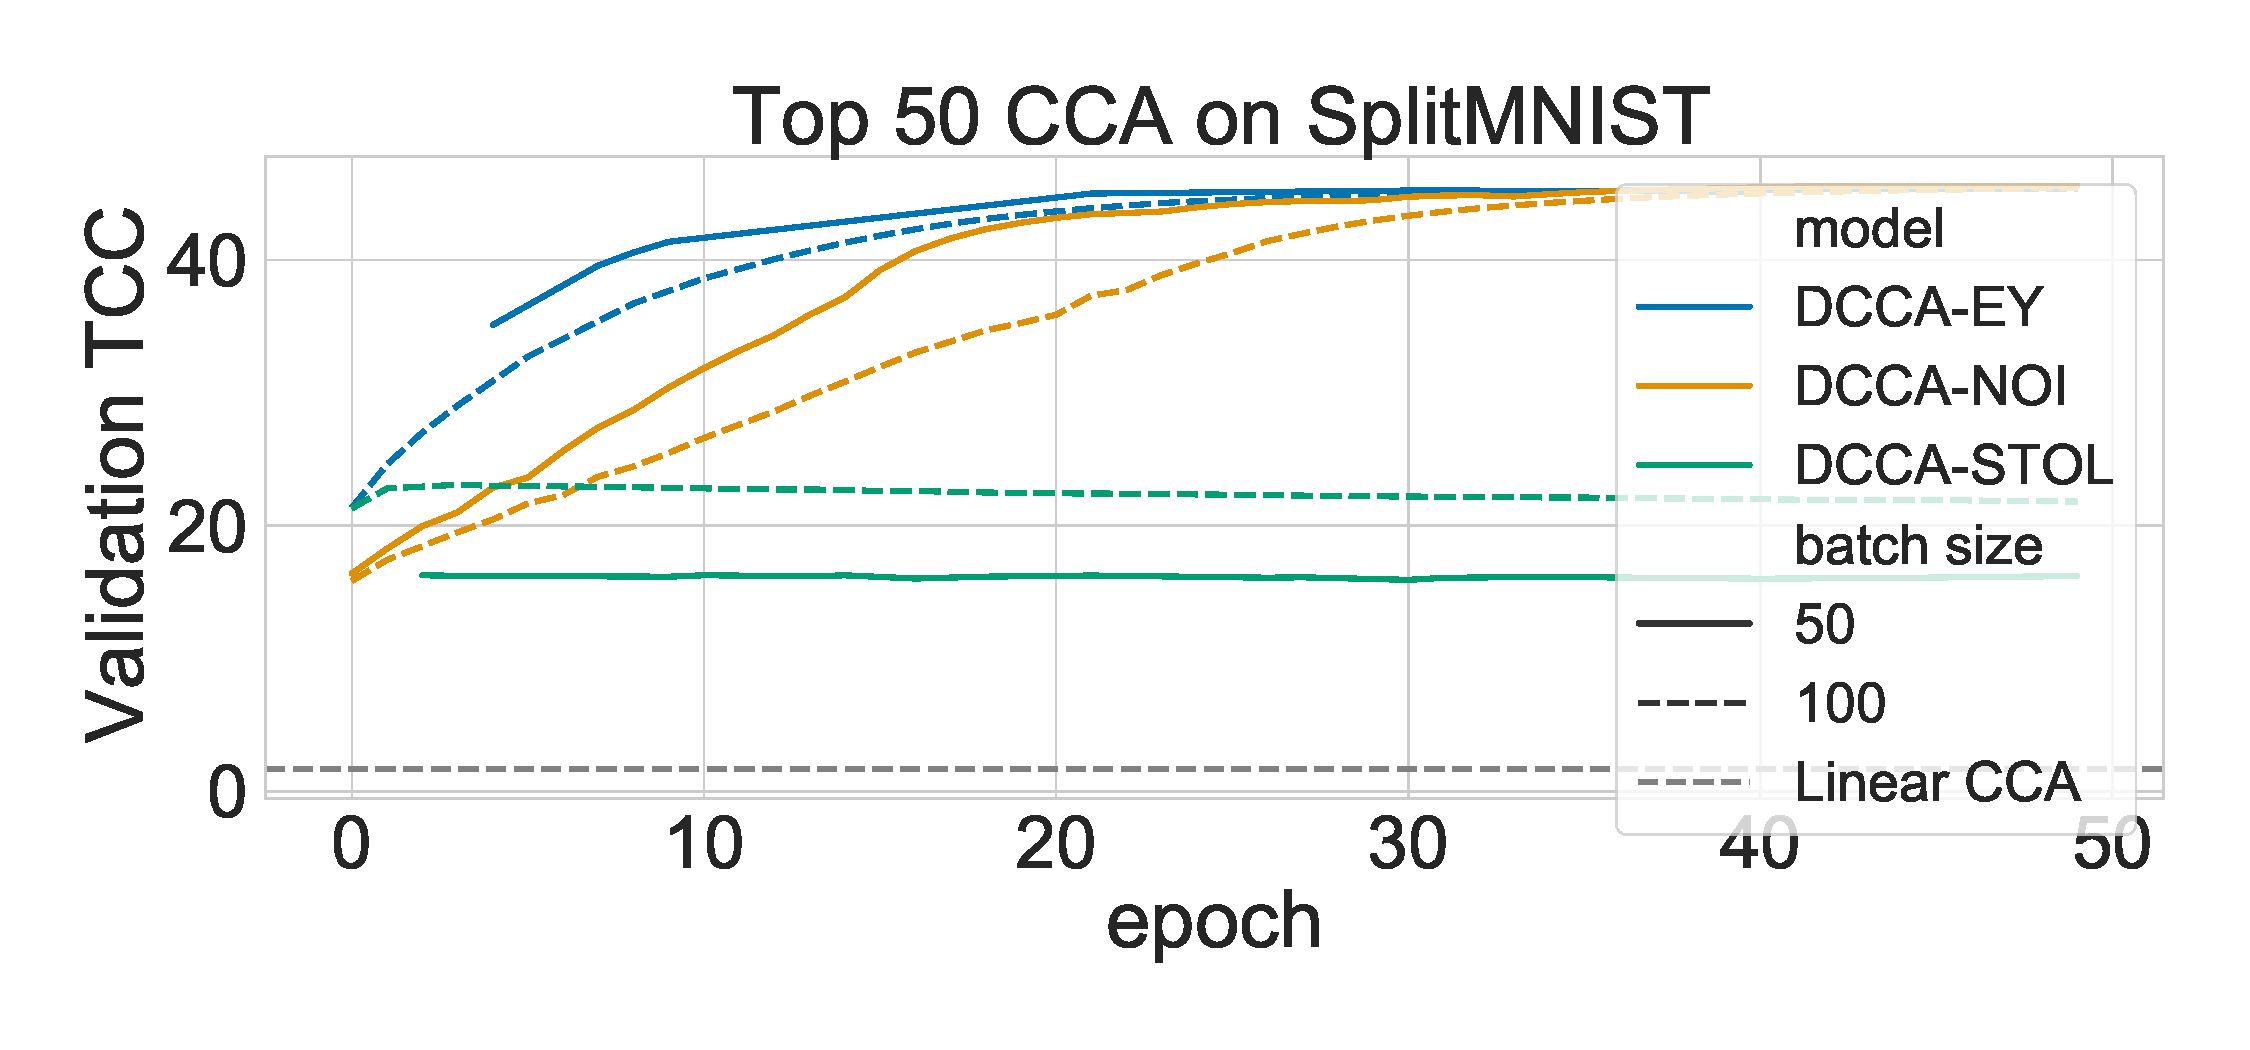
\includegraphics[width=0.8\textwidth]{figures/DCCA/SplitMNIST_allbatchsizes_pcc}
    \caption{Deep CCA on SplitMNIST: Learning progress over 50 epochs.}
    \label{fig:lr_mnist}
\end{figure}

\begin{figure}
    \centering
    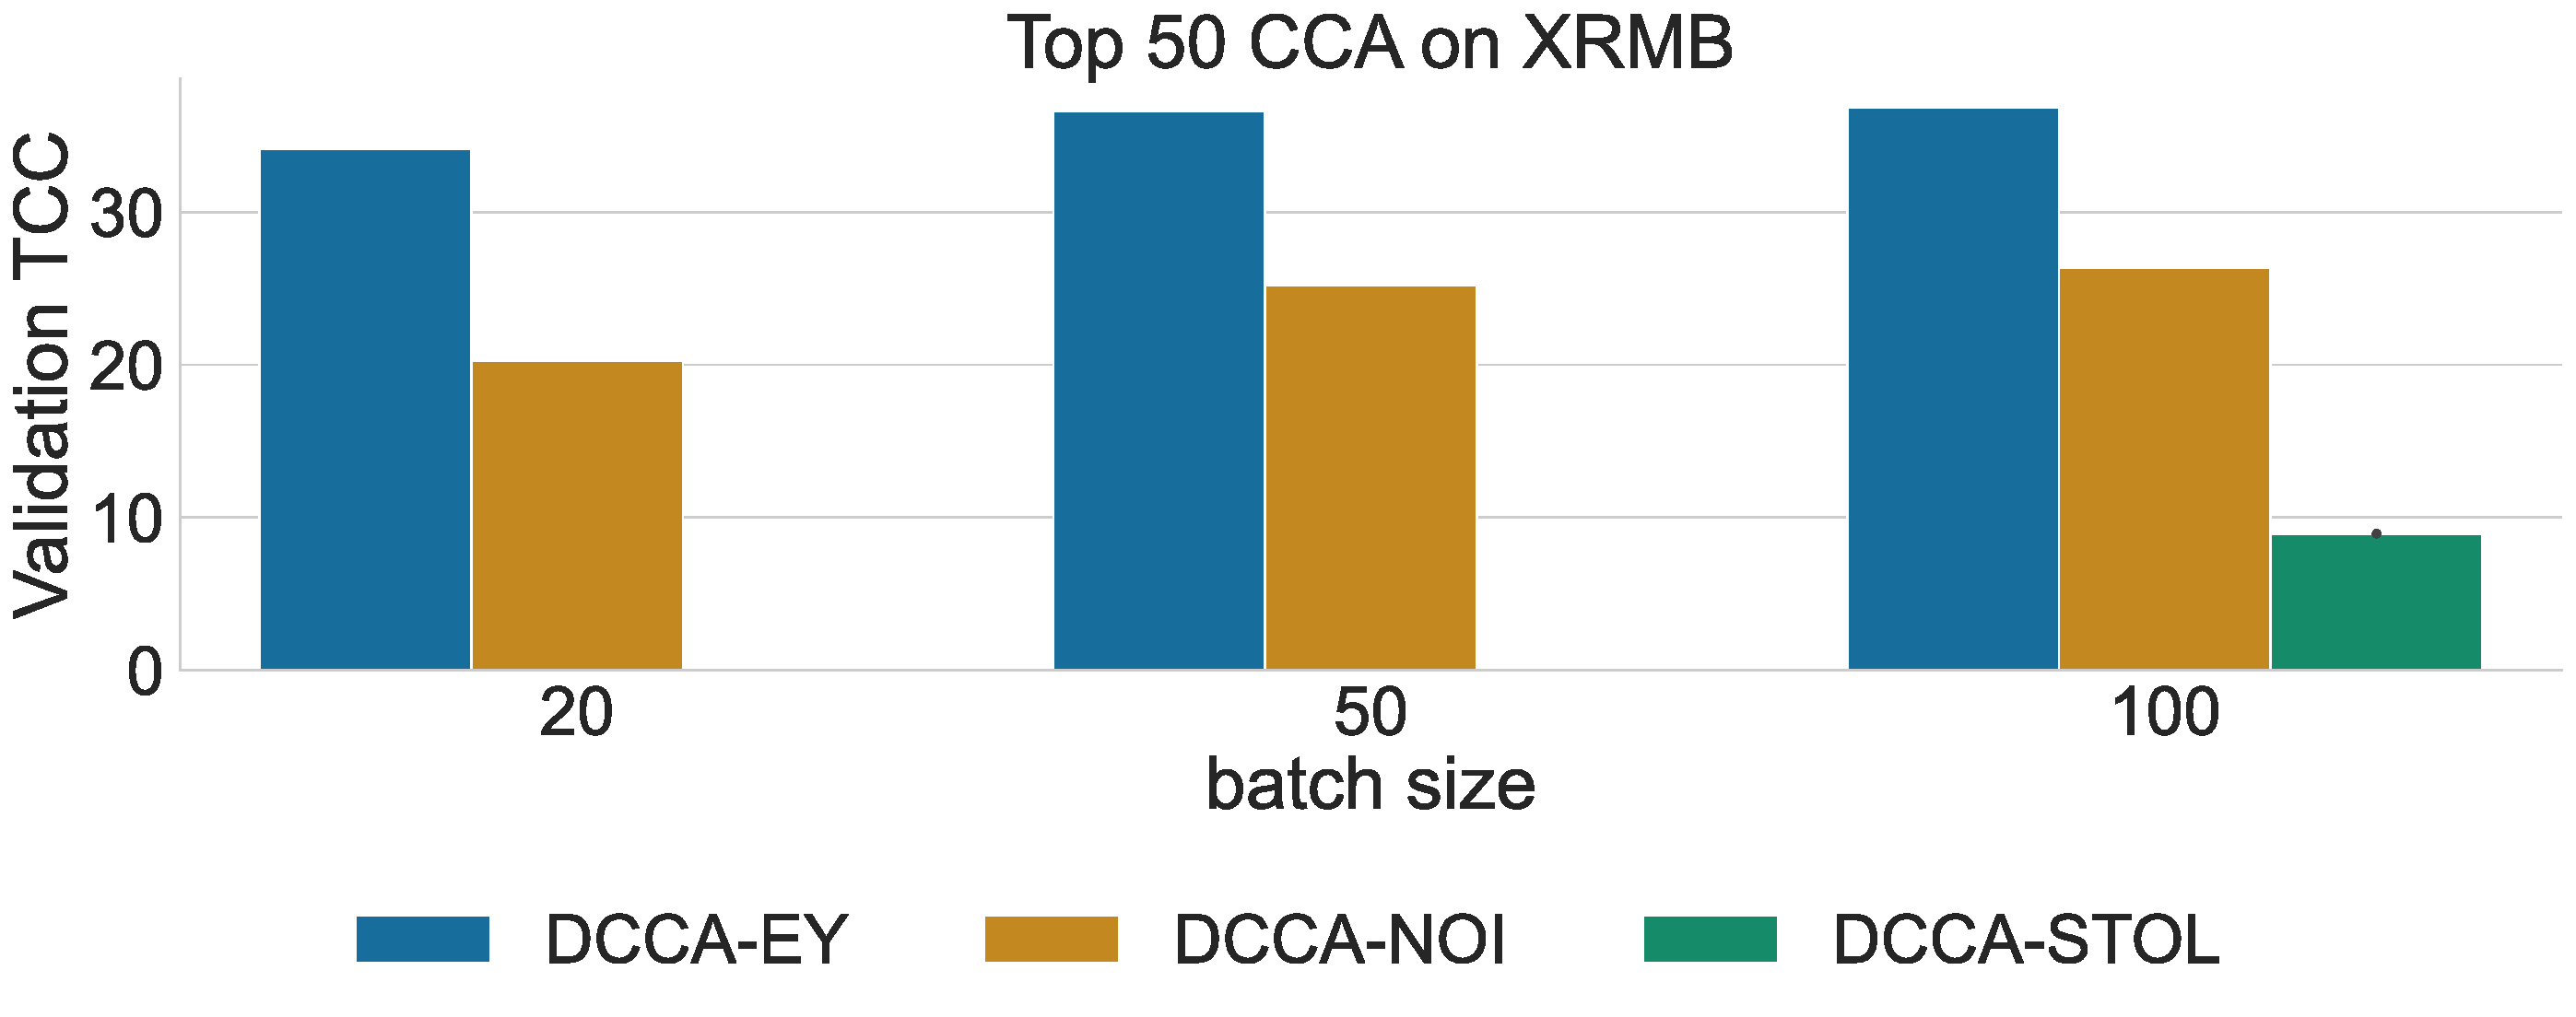
\includegraphics[width=0.8\textwidth]{figures/DCCA/XRMB_models_different_batch_sizes}
    \caption{Deep CCA on XRMB: Comparison of methods across varying batch sizes.}
    \label{fig:corr_xrmb}
\end{figure}

\begin{figure}
    \centering
    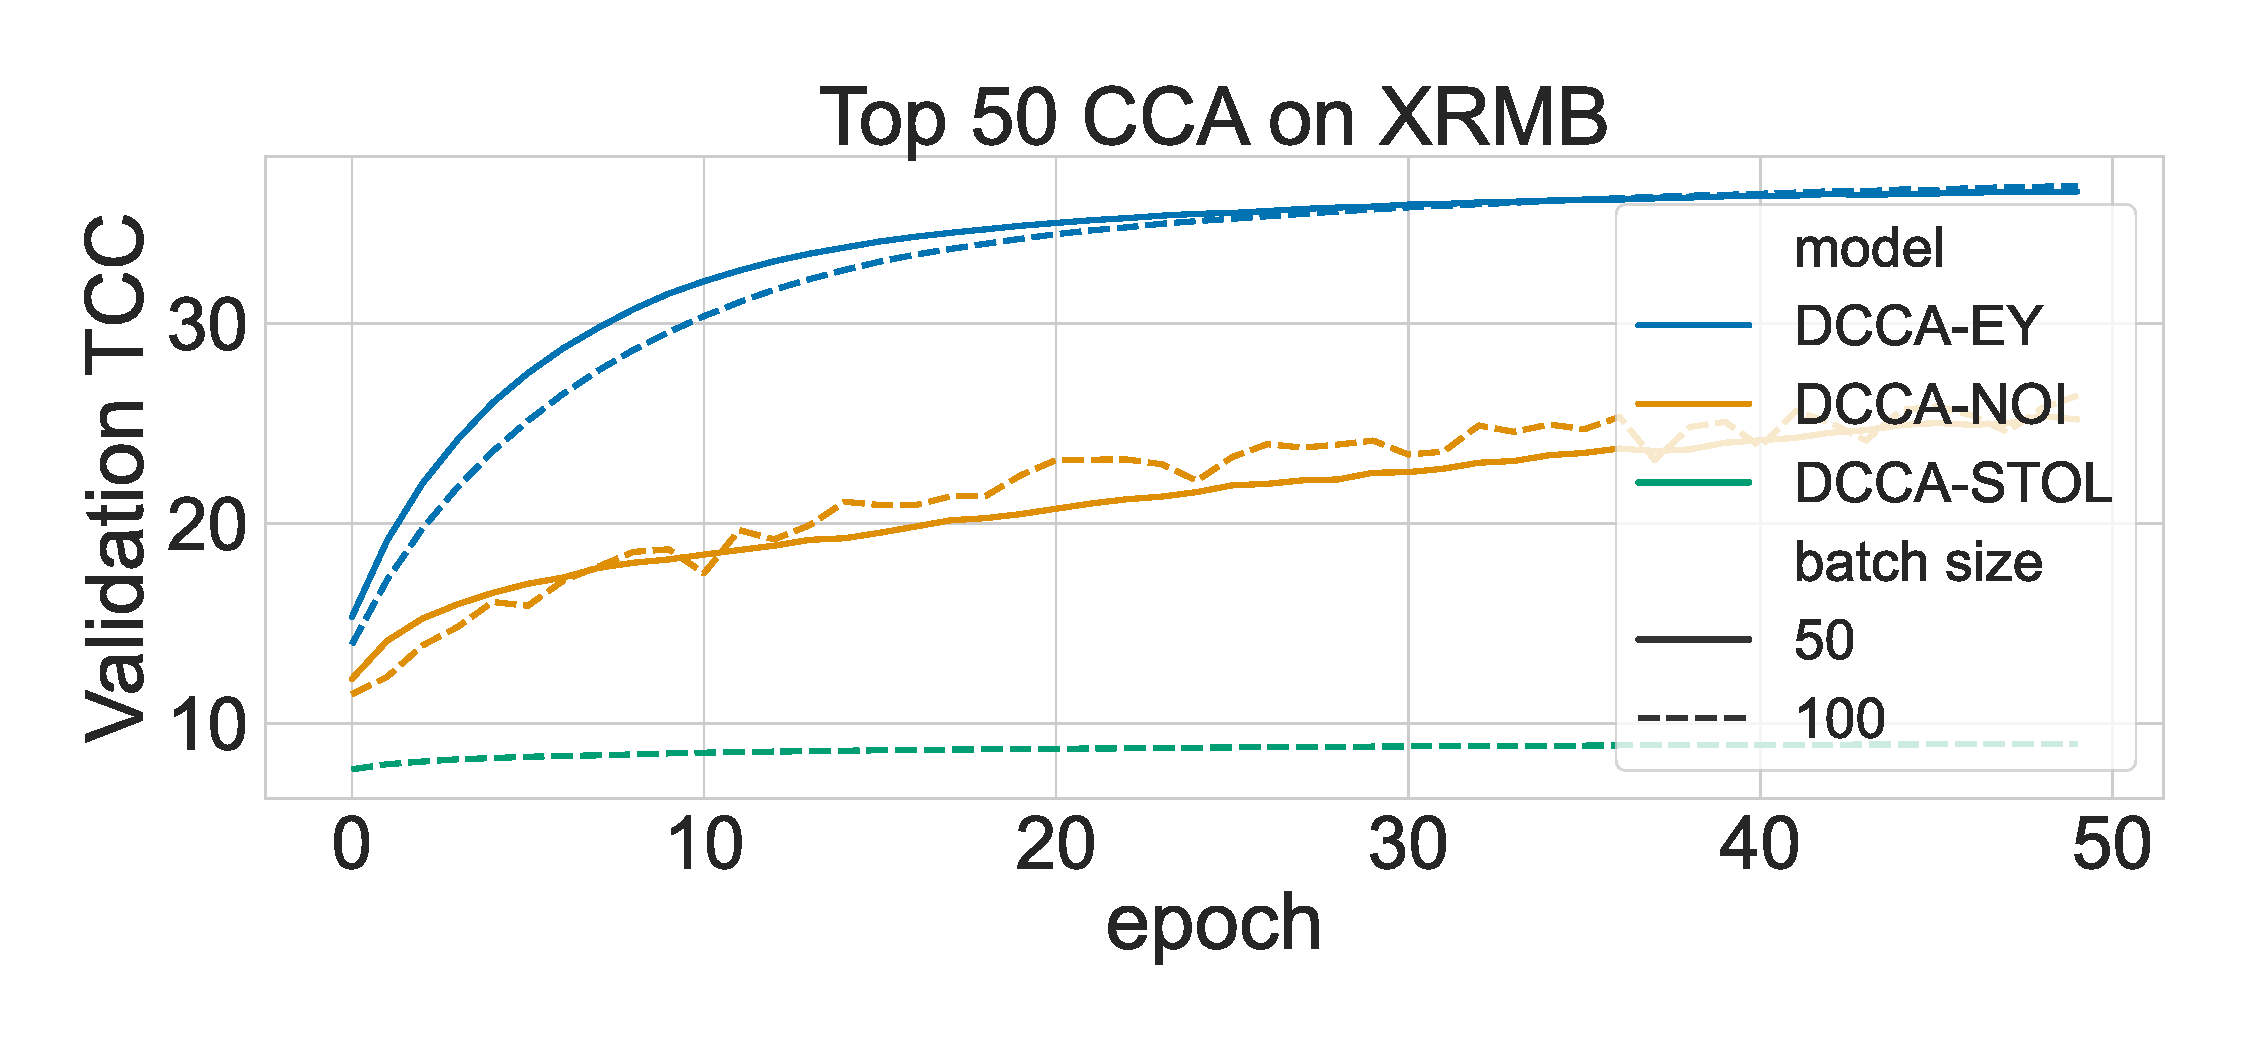
\includegraphics[width=0.8\textwidth]{figures/DCCA/XRMB_allbatchsizes_pcc}
    \caption{Deep CCA on XRMB: Learning progress over 50 epochs.}
    \label{fig:lr_xrmb}
\end{figure}

\subsection{Deep Multiview CCA: Robustness Across Different Batch Sizes}
In our second experiment, our objective is to showcase the adaptability and effectiveness of the DCCA-EY method in the multiview context, particularly in comparison to existing methods such as DMCCA and DGCCA.
We again learn $K=50$ dimensional representations, but now train for 100 epochs.
We employ a multiview extension of the Total Correlation Captured (TCC) metric, termed Total Multiview Correlation Captured (TMCC). TMCC averages the correlation across views and is defined using the consistent notation from \cref{sec:background-unified} as:
\[
    \text{TMCC} = \sum_{k=1}^{K} \frac{1}{I(I-1)} \sum_{\substack{i,j \leq I \\ i \neq j}} \text{corr}(Z_k^{(i)}, Z_k^{(j)}),
\]
where \( Z_k^{(i)} \) represents the \( k \)-th dimension of the \( i \)-th view's representation.
This metric effectively measures the extent to which our method captures correlations between different views in a multidimensional representation space.

\subsubsection{Data} We choose the mfeat dataset for this purpose, which comprises 2,000 handwritten numeral patterns represented through six distinct feature sets, including Fourier coefficients, profile correlations, Karhunen-Love coefficients, pixel averages in \(2 \times 3\) windows, Zernike moments, and morphological features.
These diverse features present an ideal testbed for evaluating the performance of multiview learning methods.

\subsubsection{Parameters} For each method, we searched over a hyperparameter grid using \citet{wandb}.

\begin{table}[h!]
    \centering
    \begin{tabular}{|l|l|}
        \hline Parameter      & Values                       \\
        \hline minibatch size & 5,10,20,50,100,200           \\
        \hline components     & 50                           \\
        \hline epochs         & 100                          \\
        \hline lr             & 0.01, 0.001, 0.0001, 0.00001 \\
        \hline
    \end{tabular}
\end{table}

\subsubsection{Observations}
Figure~\ref{fig:dmcca_corr} illustrates the comparison of DCCA-EY with DGCCA and DMCCA across different mini-batch sizes, using the validation TMCC metric.
DCCA-EY consistently outperforms both DGCCA and DMCCA, showcasing its superior ability to capture validation TMCC. Notably, DMCCA encounters issues when the batch size is smaller than $K=50$, likely due to singular empirical covariances.
DGCCA, while not breaking down, significantly underperforms with smaller batch sizes, highlighting limitations in scalability and efficiency for large-scale data applications.

In Figure~\ref{fig:dmcca_lr}, we observe the learning curves for batch sizes 50 and 100. Both DMCCA and DGCCA demonstrate rapid initial learning of significant correlations but reach a plateau relatively quickly. In contrast, DCCA-EY exhibits a consistent improvement over time and notably outperforms the other methods by the end of the training period. This behavior underscores the enhanced learning capability and efficiency of DCCA-EY, especially in the context of large-scale, high-dimensional data.

\begin{figure}
    \centering
    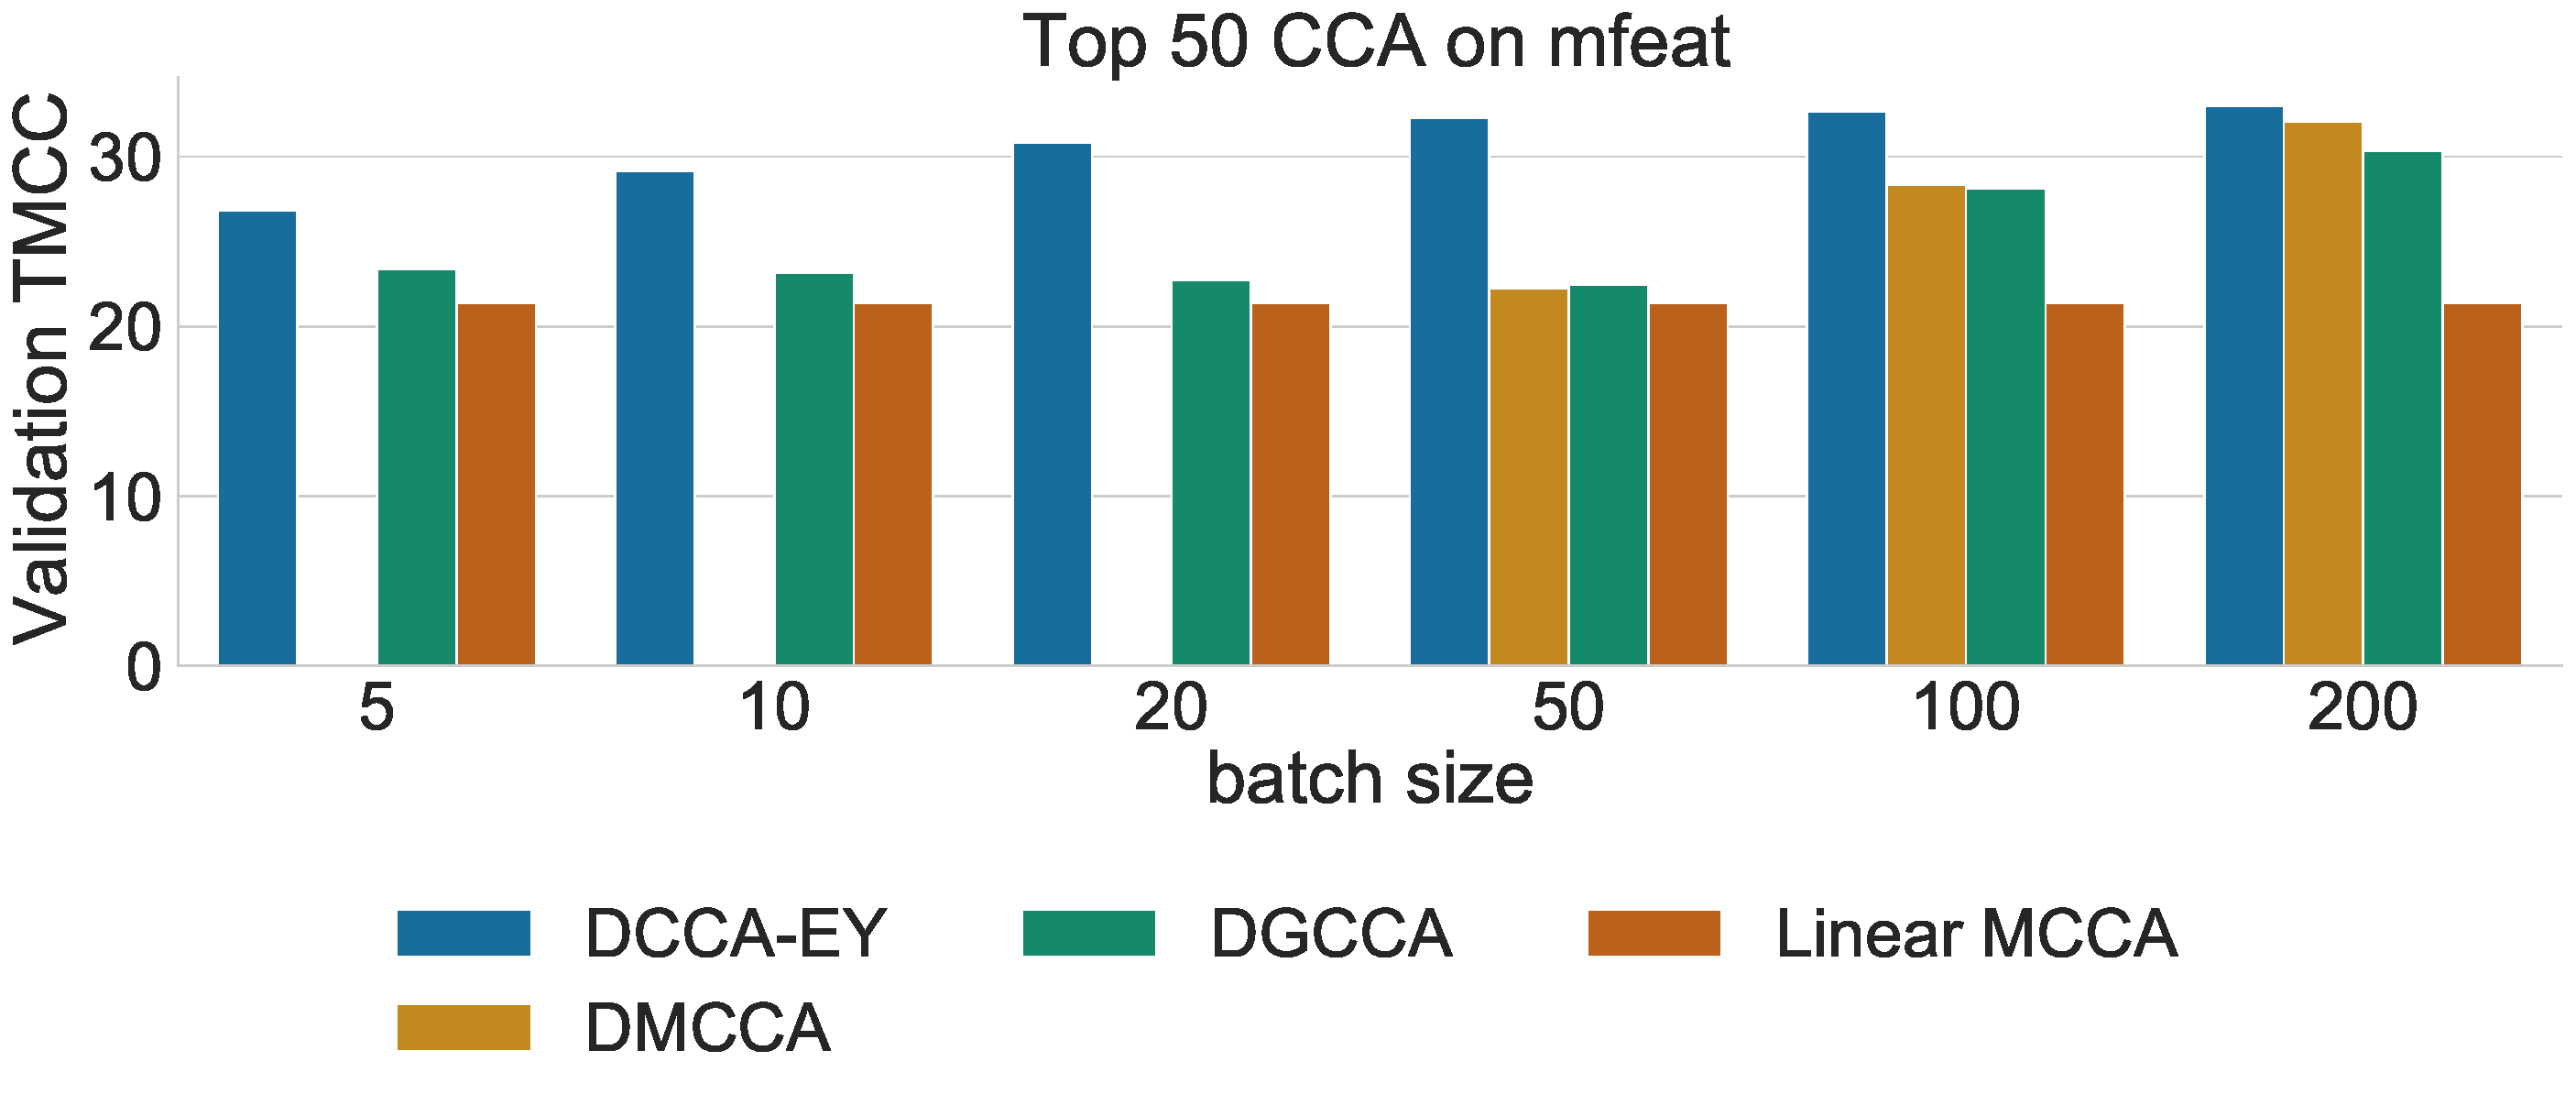
\includegraphics[width=0.8\textwidth]{figures/DMCCA/mfeat_models_different_batch_sizes}
    \caption{Deep Multi-view CCA on mfeat: Comparison across various mini-batch sizes using the Validation TMCC metric.}\label{fig:dmcca_corr}
\end{figure}

\begin{figure}
    \centering
    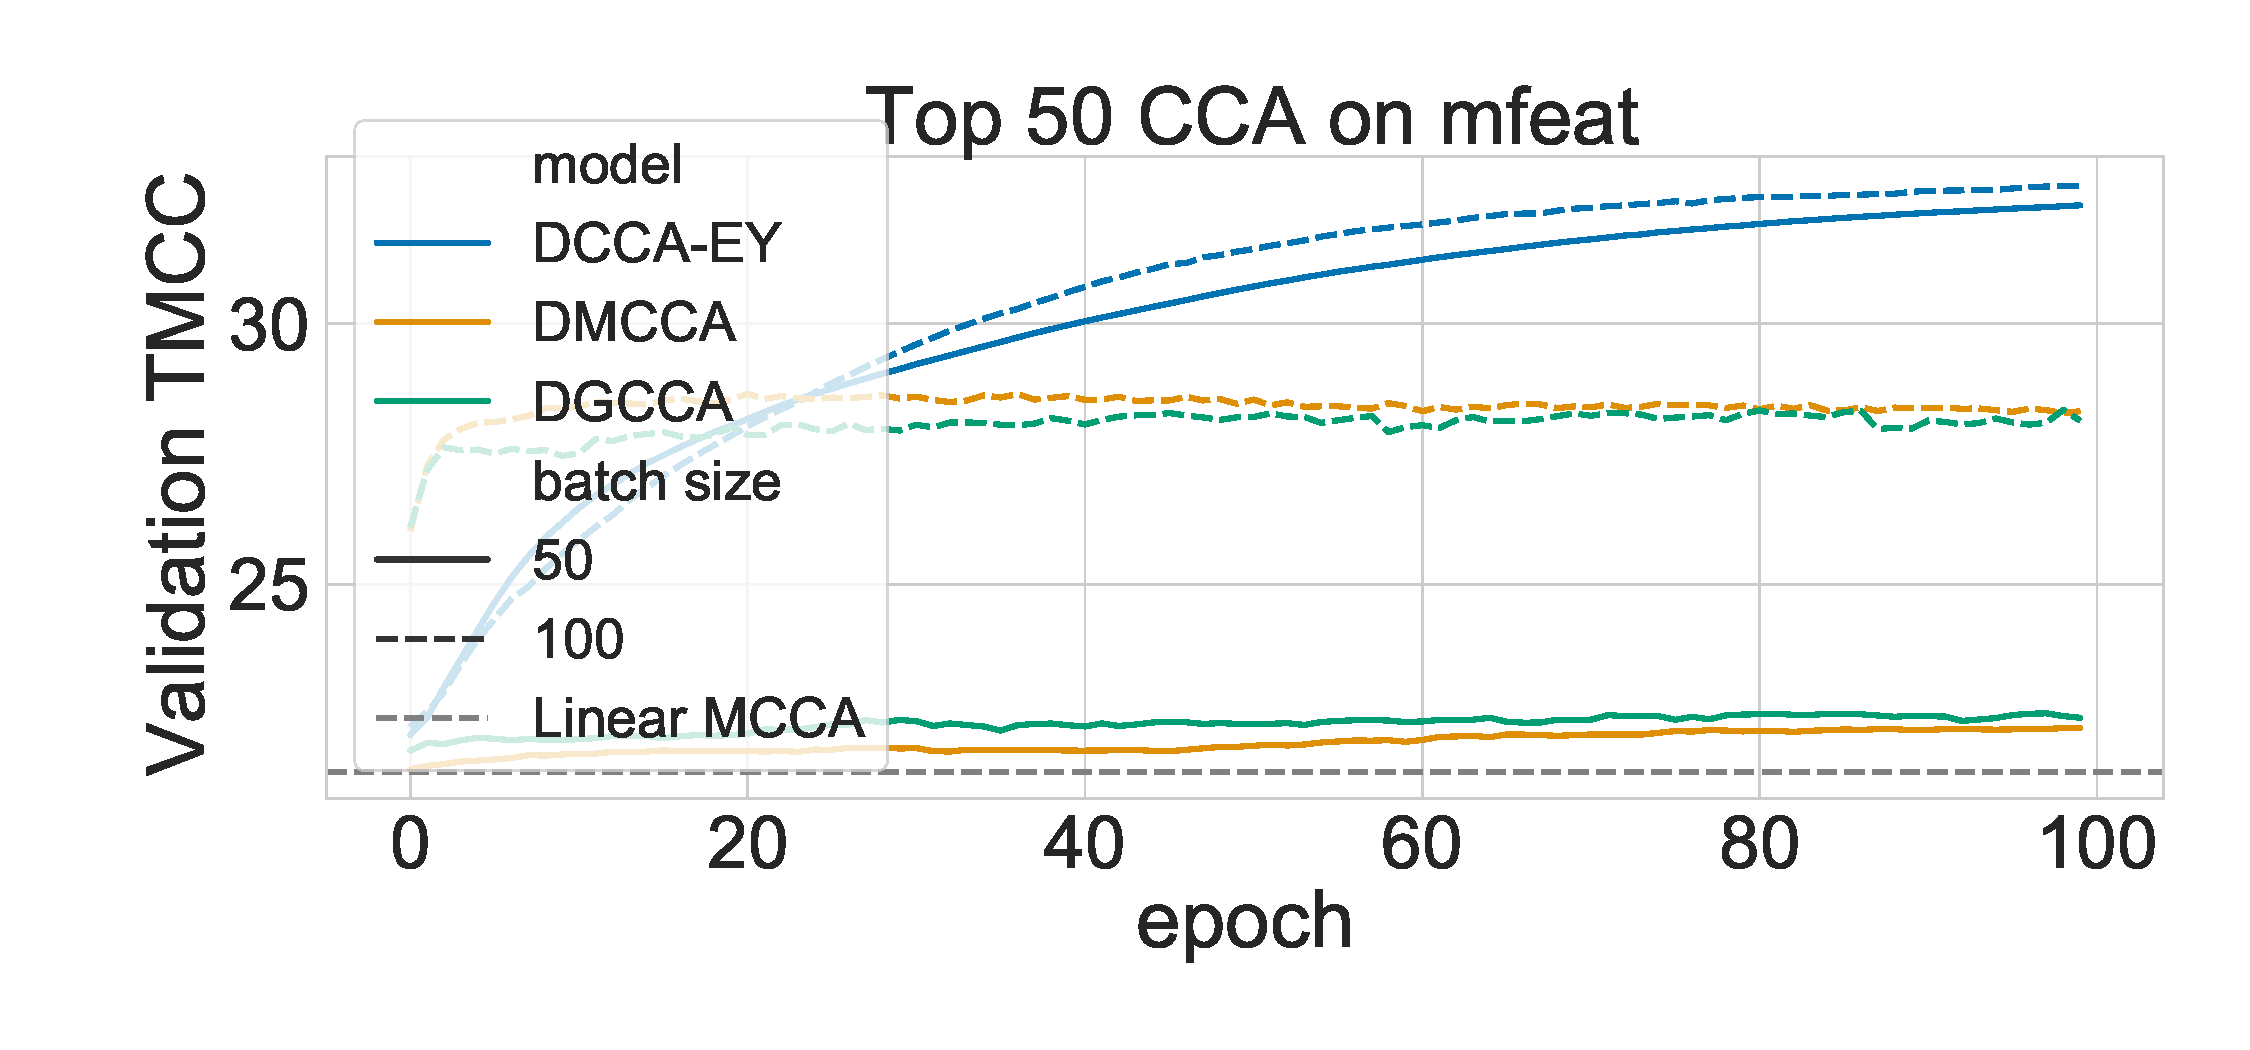
\includegraphics[width=0.8\textwidth]{figures/DMCCA/mfeat_allbatchsizes_pcc}
    \caption{Deep Multi-view CCA on mfeat: Learning progress over 100 epochs for batch sizes 50 and 100.}\label{fig:dmcca_lr}
\end{figure}

\subsection{Self-Supervised Learning with SSL-EY}
Finally, we benchmark our self-supervised learning algorithm, SSL-EY, with Barlow Twins and VICReg on standard SSL benchmarks.
We follow a standard experimental design \citep{tong2023emp}.
Indeed, we use the sololearn library \citep{da2022solo}, which offers optimized setups particularly tailored for VICReg and Barlow Twins.
All methods use a ResNet-18 encoder coupled with a bi-layer projector network.
Training spans 1,000 epochs with batches of 256 images.
For SSL-EY, we use the hyperparameters optimized for Barlow Twins, aiming not to outperform but to showcase the robustness of our method.
We predict labels via a linear probe on the learnt representations and evaluate performance with Top-1 and Top-5 accuracies on the validation set.

\subsubsection{Data} We use the CIFAR-10 and CIFAR-100 datasets, which comprise 60,000 labelled images of size 32x32.
CIFAR-10 contains 10 classes, while CIFAR-100 contains 100 classes.

\subsubsection{Observations} As Table \ref{tab:selfsup} demonstrates, SSL-EY rivals Barlow Twins and VICReg, despite employing general hyperparameters as opposed to the latter's specifically optimized ones.

\begin{table}[H]
    \centering
    \begin{tabular}{|l|c|c|c|c|}
        \hline
        Method          & CIFAR-10 Top-1 & CIFAR-10 Top-5 & CIFAR-100 Top-1 & CIFAR-100 Top-5 \\
        \hline
        Barlow Twins    & \textbf{92.1}  & 99.73          & \textbf{71.38}  & \textbf{92.32}  \\
        \hline
        VICReg          & 91.68          & 99.66          & 68.56           & 90.76           \\
        \hline
        \textbf{SSL-EY} & 91.43          & \textbf{99.75} & 67.52           & 90.17           \\
        \hline
    \end{tabular}
    \caption{Comparing the performance of SSL methods on CIFAR-10 and CIFAR-100.}
    \label{tab:selfsup}
\end{table}

\subsubsection{Model Convergence} In deep learning, a learning curve usually represents a graph showing the model's learning progress against number of epochs.
Figure \ref{fig:ssl_learning_curve_cifar100_top5} illustrates that the performance variations at 1,000 epochs, shown in Table \ref{tab:selfsup}, primarily stem from optimization noise, with convergence speeds being comparable among methods.

\begin{figure}[H]
    \centering
    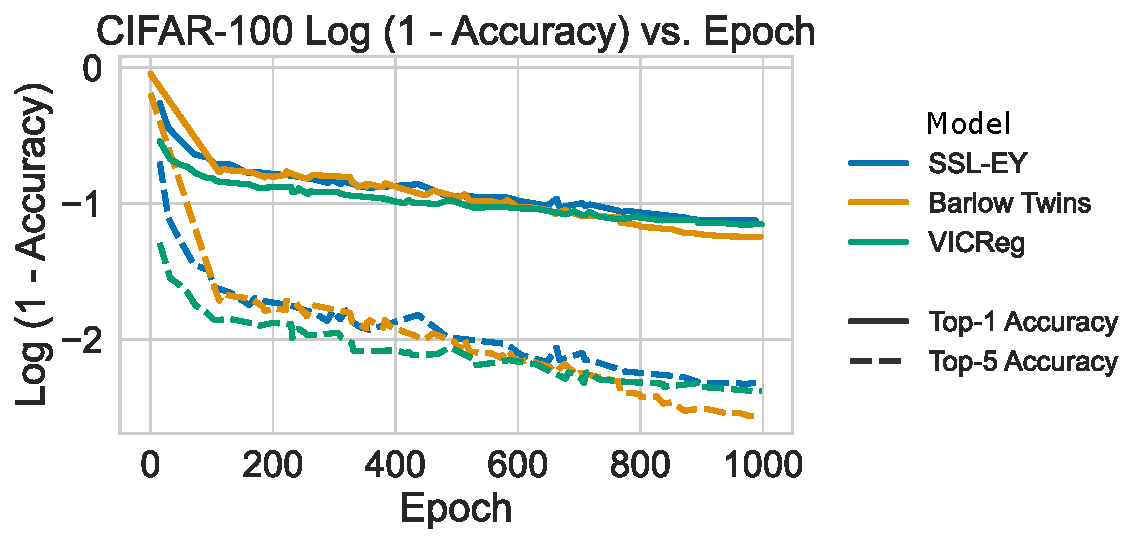
\includegraphics[width=0.8\textwidth]{figures/SSL/cifar100_learning_curve_log_error}
    \caption{Learning curves for SSL-EY, Barlow Twins, and VICReg on CIFAR-100, depicting 1,000-epoch performance.}
    \label{fig:ssl_learning_curve_cifar100_top5}
\end{figure}

\subsubsection{Projector Size Variation} We hypothesized that SSL-EY's robustness to projector size might allow for efficient performance even with smaller projectors or without one.
This hypothesis led us to experiment with varying projector output dimensions and completely removing the projector while maintaining the encoder size.
Figure \ref{fig:ssl_projector_dimensions_100} shows SSL-EY's sustained performance with reduced projector size, indicating more efficient representations compared to Barlow Twins and VICReg.
Furthermore, as Table \ref{tab:selfsup} and Figure \ref{fig:ssl_learning_curve_cifar100_vs_corr} suggest, SSL-EY performs consistently well even without a projector, underlining its reduced reliance on this architectural component.

\begin{figure}[H]
    \begin{subfigure}[b]{0.47\textwidth}
        \centering
        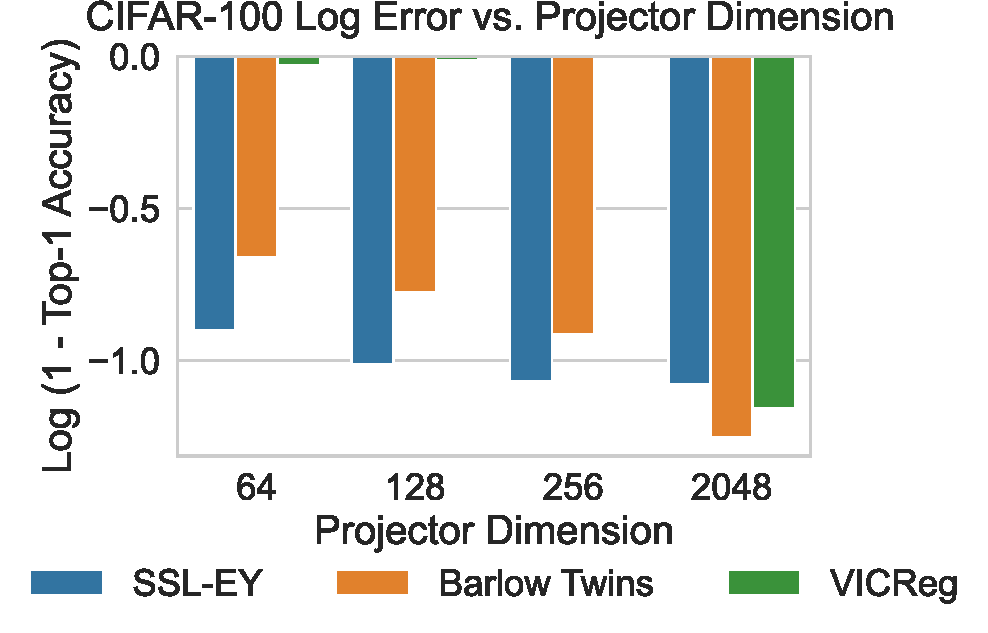
\includegraphics[width=\textwidth]{figures/SSL/cifar100_proj_dim_log_error}
        \caption{Performance of SSL-EY with varying projector dimensions on CIFAR-100.}
        \label{fig:ssl_projector_dimensions_100}
    \end{subfigure}
    \hfill
    \begin{subfigure}[b]{0.47\textwidth}
        \centering
        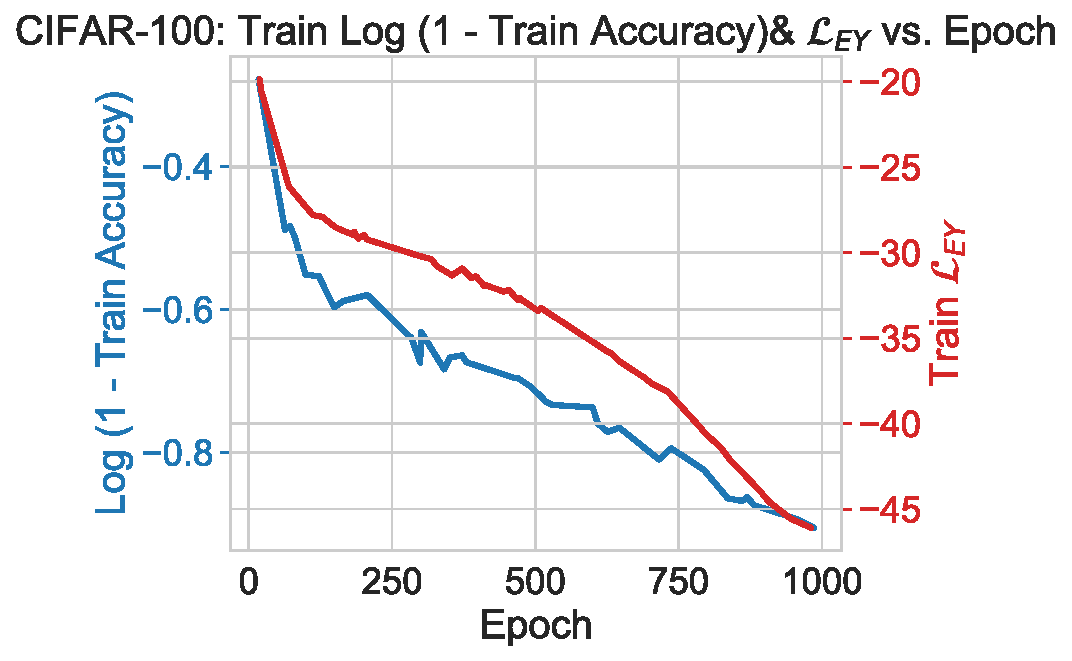
\includegraphics[width=\textwidth]{figures/SSL/cifar100_corr_vs_acc_log_error}
        \caption{Correlation of EY loss with classification accuracy in SSL-EY on CIFAR-100.}
        \label{fig:ssl_learning_curve_cifar100_vs_corr}
    \end{subfigure}
    \caption{CIFAR 100 Projector Analysis: (a) Examining the impact of projector size on SSL-EY's performance. (b) Investigating the relationship between EY loss and classification accuracy.}
    \label{fig:ssl_projector_cifar_100}
\end{figure}

\subsubsection{$\LEY$ as an Informative Metric} Figure\ref{fig:ssl_learning_curve_cifar100_vs_corr} offers two insights.
First, it evidences the close relationship between EY loss and classification accuracy, highlighting the potential of maximizing canonical correlation as a pretext task in SSL. Second, it reveals that even a reduced projector dimensionality does not reach full capacity within 1,000 epochs, implying untapped potential in SSL-EY's representation capacity.
evolution of the correlation, measured by $\LEY$, suggests a new avenue for monitoring model training, potentially eliminating the need for a separate validation task.

\begin{figure}[H]
    \centering
    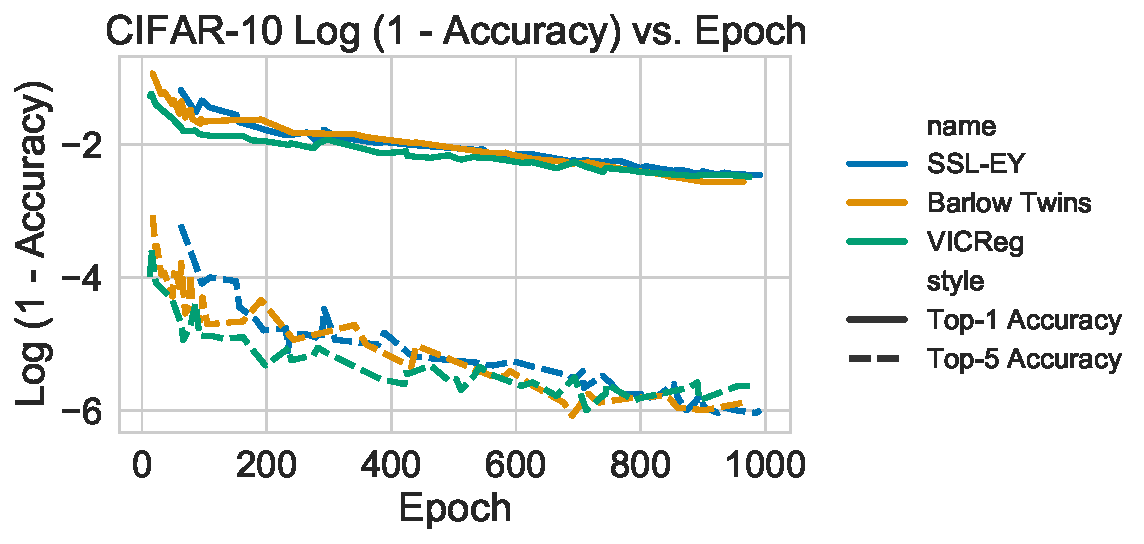
\includegraphics[width=0.57\textwidth]{figures/SSL/cifar10_learning_curve_log_error}
    \caption{Learning curves for SSL-EY, Barlow Twins, and VICReg on CIFAR-10, depicting 1,000-epoch performance.}
    \label{fig:ssl_learning_curve_cifar10_top5}
\end{figure}

\begin{figure}[H]
    \begin{subfigure}[b]{0.47\textwidth}
        \centering
        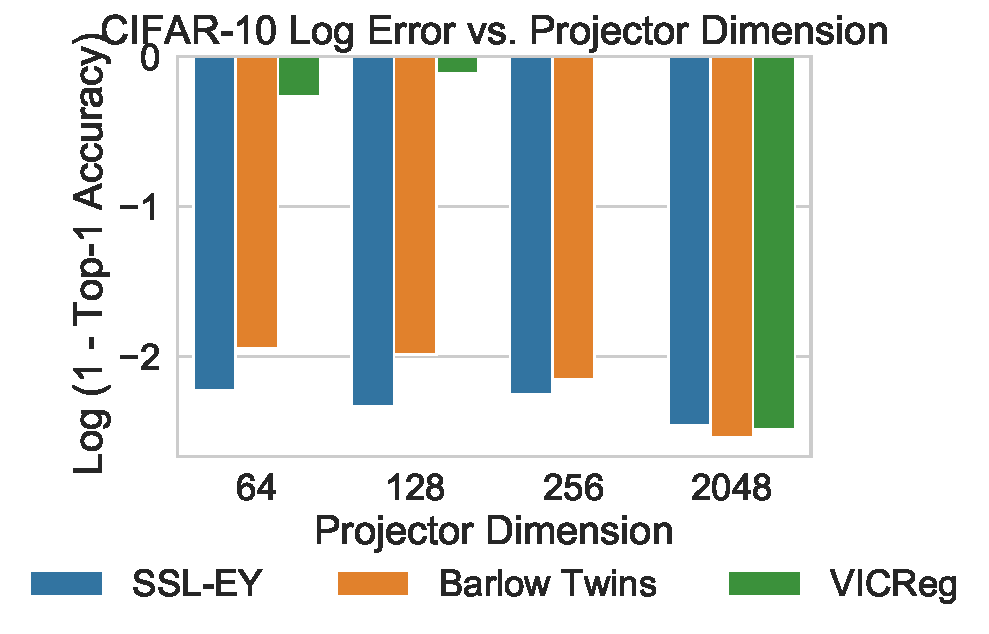
\includegraphics[width=\textwidth]{figures/SSL/cifar10_proj_dim_log_error}
        \caption{Performance of SSL-EY with varying projector dimensions on CIFAR-10.}
        \label{fig:ssl_projector_dimensions_10}
    \end{subfigure}
    \hfill
    \begin{subfigure}[b]{0.47\textwidth}
        \centering
        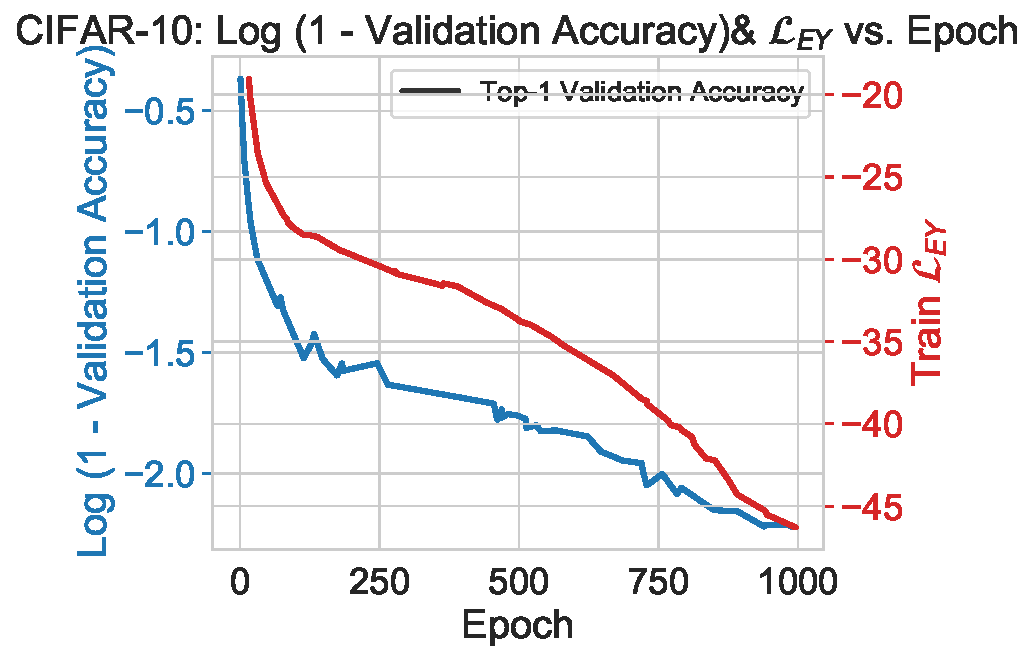
\includegraphics[width=\textwidth]{figures/SSL/cifar10_corr_vs_acc_log_error}
        \caption{Correlation of EY loss with classification accuracy in SSL-EY on CIFAR-10.}
        \label{fig:ssl_learning_curve_cifar10_vs_corr}
    \end{subfigure}
    \caption{CIFAR 10 Projector Analysis: (a) Examining the impact of projector size on SSL-EY's performance. (b) Investigating the relationship between EY loss and classification accuracy.}
    \label{fig:ssl_projector_cifar_10}
\end{figure}


\section{Discussion}

\subsection{Limitations}

Our innovative formulation of DCCA-EY successfully addresses the limitations of traditional DCCA methods, particularly in stochastic settings.
The experimental results on Split MNIST and XRMB datasets demonstrate DCCA-EY's superior capability in capturing correlations efficiently across a range of mini-batch sizes, thereby validating its scalability and robustness.
Furthermore, our method shows notable improvements in convergence speed and reduced sensitivity to hyperparameter tuning, aspects critically important for practical applications.

In SSL, SSL-EY stands out as a competitive and robust approach.
Our experiments on CIFAR-10 and CIFAR-100 highlight SSL-EY's ability to achieve comparable performance with state-of-the-art methods like Barlow Twins and VICReg, even while using general hyperparameters.
This is important given the time it takes to run experiments with SSL methods which, as here, can be up to 1,000 epochs.
This underscores SSL-EY's adaptability and robustness in different settings.
Particularly noteworthy is its performance with reduced or absent projectors, indicating its efficiency and potential for broader applications in SSL\@.
Moreover, the insights gleaned from the correlation of EY loss with classification accuracy in SSL-EY open new avenues for understanding and leveraging canonical correlations in SSL. The observed relationships provide a promising direction for future research in developing more effective and efficient SSL methods.

\subsection{Conclusion}

Our work bridges significant gaps in the literature and establishes a strong foundation for future explorations in both DCCA and SSL. The proposed methods not only enhance our understanding of these domains but also pave the way for practical applications where scalability, efficiency, and robustness are paramount.
In summary, this chapter contributes to the advancement of DCCA and SSL by introducing novel approaches that are not only theoretically sound but also practically viable, offering valuable tools for researchers and practitioners alike in the ever-evolving landscape of machine learning.